\documentclass{article}

% if you need to pass options to natbib, use, e.g.:
%     \PassOptionsToPackage{numbers, compress}{natbib}
% before loading aaj2026


% ready for submission
\usepackage[final]{aaj2026}
\bibliographystyle{IEEEtran}
% use CJKutf8 for Chinese characters; scheme=plain keeps caption names (Figure/Table/Contents) in English
\usepackage[scheme=plain]{ctex}

% to compile a preprint version, e.g., for submission to arXiv, add add the
% [preprint] option:
%     \usepackage[preprint]{aaj2026}


% to compile a camera-ready version, add the [final] option, e.g.:
%     \usepackage[final]{aaj2026}


% to avoid loading the natbib package, add option nonatbib:
%    \usepackage[nonatbib]{aaj2026}


\usepackage[utf8]{inputenc} % allow utf-8 input
\usepackage[T1]{fontenc}    % use 8-bit T1 fonts
\usepackage{hyperref}       % hyperlinks
\usepackage{url}            % simple URL typesetting
\usepackage{booktabs}       % professional-quality tables
\usepackage{amsfonts}       % blackboard math symbols
\usepackage{nicefrac}       % compact symbols for 1/2, etc.
\usepackage{microtype}      % microtypography
\usepackage[table]{xcolor}         % colors
\usepackage[most]{tcolorbox} % colored boxes
\usepackage{graphicx}       % graphics
\usepackage{tikz}
\usepackage{caption}
\usepackage{makecell}
\usepackage{setspace}
\onehalfspacing
\definecolor{coverlinecolor}{HTML}{002FA7}
\newcommand{\foo}{\color{coverlinecolor}\makebox[0pt]{\textbullet}\hskip-0.5pt\vrule width 1pt\hspace{\labelsep}}
\usetikzlibrary{arrows.meta, positioning, shapes.geometric, calc}

\title{Topological Feature Analysis of Focus Music Based on Path Homology and Its Application in ACE-Step Latent Space Guided Generation}


% The \author macro works with any number of authors. There are two commands
% used to separate the names and addresses of multiple authors: \And and \AND.
%
% Using \And between authors leaves it to LaTeX to determine where to break the
% lines. Using \AND forces a line break at that point. So, if LaTeX puts 3 of 4
% authors names on the first line, and the last on the second line, try using
% \AND instead of \And before the third author name.


\author{%
  Fisher E. Yu \\
  \texttt{September 12, 2026} \\
}


% Close the page anchor on the information page to avoid duplicating the page number of the first page of the main text
\hypersetup{pageanchor=false}

\begin{document}

% ======== Contest Information Page (not counted in the main-text page numbering, DO NOT TRANSLATE) ========
\thispagestyle{empty}
\begin{center}
  \vspace*{3cm}
%   {\zihao{2}\heiti 参赛信息页\par}
%   \vspace{2cm}
  \renewcommand{\arraystretch}{2.2}
  {\zihao{3}
  \begin{tabular}{r@{：}l}
    参赛学生姓名 & \underline{\makebox[9cm][l]{于儿 \; Fisher E. Yu}} \\
    中学         & \underline{\makebox[9cm][l]{华南师范大学附属中学}} \\
    省份         & \underline{\makebox[9cm][l]{广东省}} \\
    国家/地区    & \underline{\makebox[9cm][l]{中国}} \\
    指导老师姓名 & \underline{\makebox[9cm][l]{杨晓安，肖天昂}} \\
    指导老师单位 & \underline{\makebox[9cm][l]{华南师范大学附属中学，谱蓝云}} \\
    论文题目     & \parbox[t]{9cm}{%
        \linespread{1.5}\selectfont
      \underline{\makebox[9cm][l]{Topological Feature Analysis of Focus}}\\
      \underline{\makebox[9cm][l]{Music Based on Path Homology and Its}}\\
      \underline{\makebox[9cm][l]{Application in ACE-Step Latent Space}}\\
      \underline{\makebox[9cm][l]{Guided Generation}}%
    } \\
  \end{tabular}}
\end{center}
\clearpage
\setcounter{page}{1}
\hypersetup{pageanchor=true}
% ======== End of Contest Information Page ========

\maketitle


\begin{abstract}
  Functional focus music is widely used in study and work settings, but the temporal structure that distinguishes it from general music still lacks a representation that is computable, auditable, and usable for generation control. This paper models music as a directed dynamical system that evolves over time. On a dataset of $300$ Open Focus and $300$ Classical instrumental tracks with per-track provenance and license records, we follow a ``discovery fitting, freezing, primary validation, duration sensitivity'' pipeline and combine GLMY path homology with phase-lifted path homology to compare local state transitions and cross-period phase closure. The primary analysis on validation/180s shows that $13/20$ and $14/20$ prespecified metrics pass BH-FDR for the pitch and rhythm views, respectively; Classical generally exhibits broader state coverage and transition diversity, whereas Open Focus exhibits a higher self-transition ratio and directed recurrence rate. The modulation view has $5/20$ metrics passing the primary-analysis FDR, but because its SMP-$K=10$ representation was proposed after the holdout was opened, it is interpreted only as exploratory evidence. None of the three local views yields a stable between-group difference in $H_1$. At the macro scale, the Acoustic and Chroma phase \texttt{loop\_score} values of Open Focus are higher than those of Classical, with rank-biserial effect sizes of $0.459$ and $0.338$, and both pass the three-view BH-FDR; Rhythm phase does not pass FDR at the primary scale. Multi-scale analysis shows between-group distance differences in the Pitch, Phase, and joint spaces, but the joint representation does not outperform the best single block. Based on these results, we freeze an $18$-dimensional fingerprint for subsequent unseen data and generation experiments, consisting of a $16$-dimensional Pitch block together with one dimension each from Acoustic phase and Chroma phase, with squared-distance weights of $1/2:1/4:1/4$. Furthermore, we implement an inference-time guidance protocol on ACE-Step 1.5 that follows an ``exact Path Homology teacher, differentiable latent-space surrogate, exact re-verification'' design: a surrogate network is trained to predict the exact topological labels of the clean latent variables at every sampling step, and it completes and passes coordinate prediction, candidate ranking, uncertainty calibration, and OOD/no-op qualification tests on unseen prompts, seed families, and generation trajectories, after which the final evaluation is conducted on $512$ paired baseline/guided audio clips. This evaluation takes the frozen exact topological target band as the primary endpoint and includes prompt consistency, audio quality, diversity, runtime, and memory overhead as prespecified non-inferiority criteria, thereby forming a complete chain of evidence from observational structure discovery and fingerprint freezing to gated generation evaluation. The conclusions of this paper concern only the topological structure representation and generation control under the current corpus and frozen protocol, and do not support causal claims about attention improvement or clinical efficacy.
\end{abstract}


\begin{keywords}
  Focus Music, Topological Music Analysis, Path Homology, Persistent Path Homology, Topology-Guided Music Generation, Latent Topology Surrogate Network, ACE-Step
\end{keywords}

\clearpage

\setcounter{tocdepth}{2}
\tableofcontents

\clearpage

\section{Introduction}

% Research background
Attention Deficit Hyperactivity Disorder (ADHD) is a common neurodevelopmental disorder, with a global prevalence of about $7$--$10\%$ in children and about $2$--$5\%$ in adults \cite{Siva2025}. By conservative estimates, roughly 240 million people are affected by attention deficits in the world. In scenarios such as studying, writing, programming, and deep work, focus music is often used to support sustained attention. Studies have shown that purposefully designed focus music has remarkable potential for assisting attention \cite{MADJAR2020113207, Phoebe2025, Erarslan2026}.

In recent years, with the development of EEG, fMRI, and large language models, more and more researches have begun to examine the relationship between the acoustic features of functional music and attention scenarios. For example, Kevin J. P. Woods et al. systematically investigated how the amplitude modulation (AM) properties of music affect sustained attention \cite{Woods2024}. Through large-scale analysis of Reddit data with the Spotify API and large language models, Achuthan et al. revealed differences in acoustic features among focus music, stuck songs, and general purpose music \cite{Achuthan2025}.

% Limitations of prior work
However, many music feature studies based on data statistics or topological data analysis (TDA) ignore the order of music events. In music theory, the transition sequence of notes or chords has an absolute temporal direction. For example, ``C major $\to$ G major'' and ``G major $\to$ C major'' differ fundamentally at the auditory and psychological levels. Order and context are important components of musical expectation \cite{Stefan2000, David2001}, and maintaining auditory expectation is a primary mechanism for avoiding distraction \cite{Fiedlere2066232025}.

% Research goal and methods
This paper argues that the transition direction should be explicitly preserved when analyzing the dynamic organization of music. Therefore, we introduce GLMY path homology \cite{glmy2013,glmy2020} and persistent path homology \cite{Samir2017} to compare the Open Focus and Classical groups in terms of local directed state transitions and cross-period phase closure. The goal of this study is to obtain a topological structure representation that is computable, auditable, and further usable for generation control, and then to apply it to the generation of focus music.

\begin{tcolorbox}[colback=pink!15,colframe=pink!50,boxrule=0.5pt,arc=6pt,left=6pt,right=6pt,top=4pt,bottom=4pt]
This paper DOES NOT evaluate attention, learning outcomes, or clinical efficacy. Even if the generated audio is closer to the frozen topological fingerprint, it cannot be inferred that it has a therapeutic effect on ADHD or other attention disorders.
\end{tcolorbox}

This study consists of two stages. The first stage fits and freezes the representation on the discovery dataset, performs the primary evaluation on validation/180s, and checks duration sensitivity using validation/300s of the same tracks; these steps yield an $18$-dimensional Path Homology fingerprint. The second stage proposes an ``exact teacher, differentiable surrogate, exact re-verification'' generation protocol for ACE-Step 1.5 \cite{gong2026}. The overall analysis and application framework are shown in Figure~\ref{fig:p1}. The framework does not presuppose any feature of Focus Music, nor does it treat the maximization or minimization of any topological metric as the generation objective; instead, it attempts to characterize the structural balance that music forms between local connectivity and periodic return.

\begin{figure}[htbp]
    \centering
    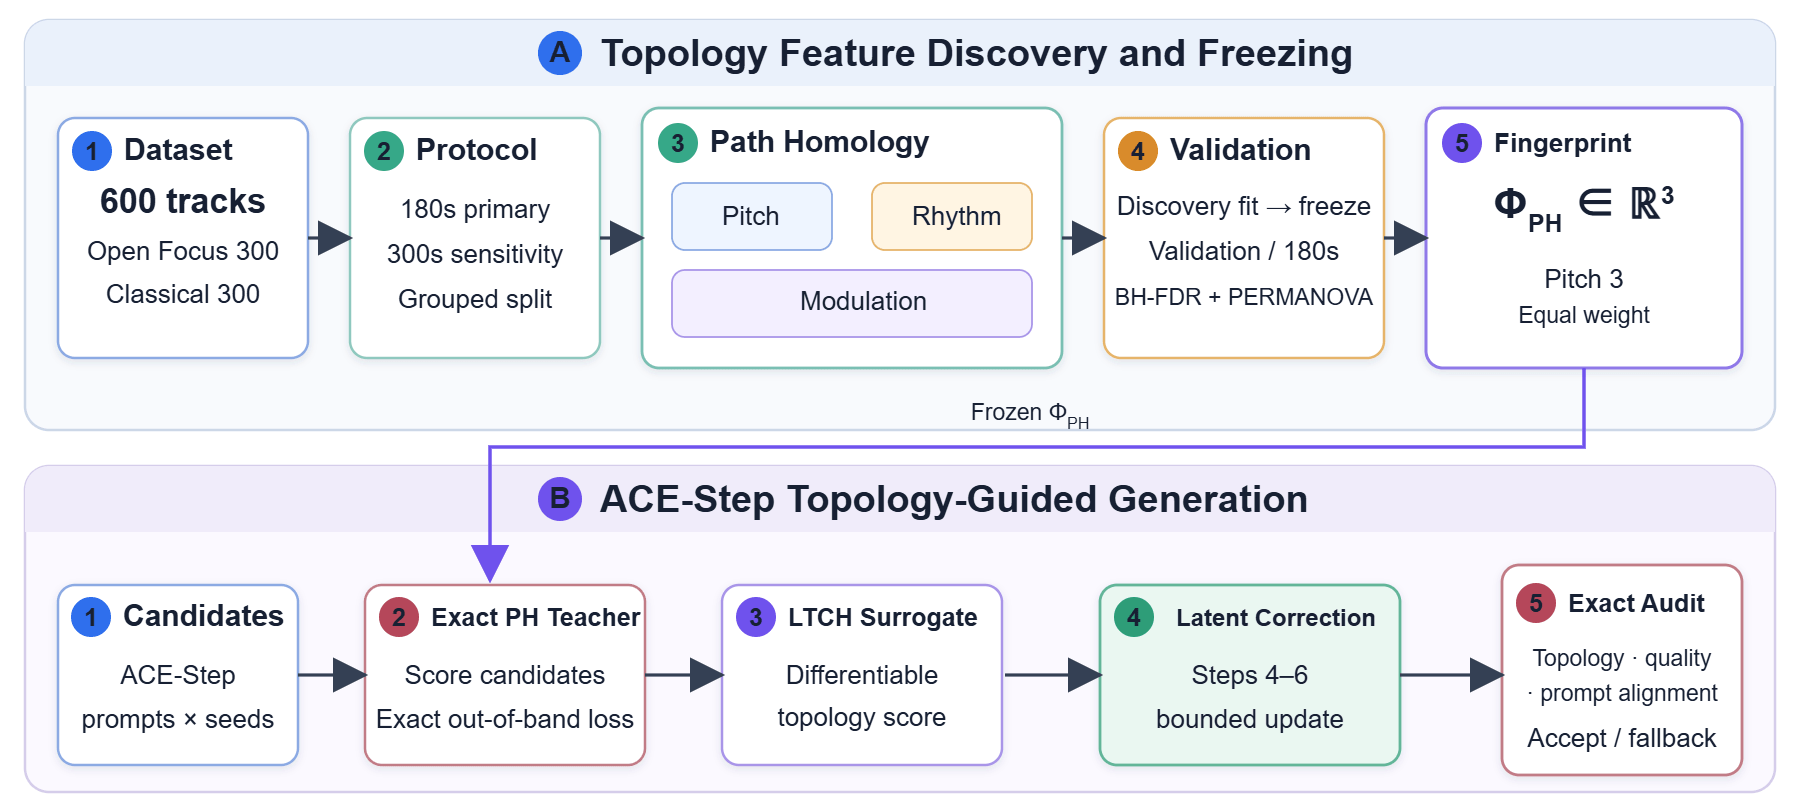
\includegraphics[width=\textwidth]{fig/p1.png}
    \caption{Overall analysis and application framework.}
    \label{fig:p1}
\end{figure}

% Key Contributions
The main contributions of this study are summarized as follows:

\begin{itemize}
  \item We construct a multi-scale analysis framework that preserves transition direction. Musical state transitions are represented as directed graphs, GLMY path homology and persistent path homology are used to analyze the topological features of music, and the observational differences between Open Focus and Classical are evaluated.
  \item We propose a phase-lifted recurrence graph representation, in which the edge weights of a six-phase directed cycle are defined by same-phase recurrence across periods, and the closure strength is characterized by the persistence threshold of the weakest edge.
  \item We organize the evidence as ``discovery fitting and freezing, validation/180s primary evaluation, and validation/300s same-track sensitivity analysis'', and freeze an $18$-dimensional topological fingerprint composed of Pitch, Acoustic phase, and Chroma phase.
  \item We propose and train a Latent Topology Surrogate Network (LTSN) that learns a differentiable approximation from ACE-Step latent variables to the frozen topological fingerprint, providing gradients for latent correction during sampling.
  \item We build a dual-scale corpus with auditable provenance and per-track licenses, containing 300 Open Focus and 300 Classical tracks, each provided with both 180s and 300s analysis segments. Available at \url{https://huggingface.co/datasets/fisheryv/open-focus-classical-600}
  \item We package the code used in the topological feature discovery process into a Python library named \texttt{pyglmy}, available at \url{https://github.com/fisheryv/pyglmy}.
\end{itemize}

% The fully reproducible code of this study has been uploaded to \url{https://github.com/fisheryv/glmy_focus_music}.

\section{Related Work}

\subsection{Topological Analysis of Music}

The Tonnetz is one of the important geometric representations of music, and its subsequent generalizations can be used to express pitch-class, interval, and temporal relationships \cite{Yust2020}. Mazzola's \emph{The Topos of Music} establishes a broader mathematical framework for music theory from the perspectives of categories, modules, and topology \cite{Guerino2017}. These works show that musical relations can be organized into spatial or algebraic structures, but they do not directly provide the directed temporal statistics required by this paper.

In topological data analysis (TDA), persistent homology tracks the appearance and disappearance of topological features across scales through a family of filtered complexes \cite{Edelsbrunner2002}. Here, $H_0$ describes connected components, $H_1$ describes loops, and $H_2$ describes two-dimensional cavities. Persistence diagrams \cite{David2007} and barcodes \cite{Carlsson2004} are common summary forms of the same persistence information. In music research, Sethares and Budney demonstrated loop structures in pitch, interval, and rhythm that can be revealed by topological methods \cite{Sethares_2014}. Alcal\'a-Alvarez and Padilla-Longoria proposed a systematic analysis framework from score point sets to simplicial complexes \cite{Alberto2024}. Heo et al. further compared the influence of different network distances on persistent homology of music network \cite{Heo_2025}. Together, these studies show that the results depend on the choice of representation and distance, and no single topological summary should be regarded as a representation-independent essence of music.

However, the standard Vietoris--Rips complex is undirected and symmetric, a limitation that prevents it from being effectively applied to directed graphs. To address the homology computation of directed graphs, Alexander Grigor'yan, Yong Lin, Yuri Muranov, and Shing-Tung Yau proposed the path complex and path homology \cite{glmy2013, glmy2020}. Mijangos et al. represented interval transitions as graphs and used persistent homology to explore differences in musical style \cite{Martin2022}, and Wei studied the acoustic shape of instruments from topological and spectral perspectives \cite{Wei2024}. Compared with TDA, GLMY path homology is still rarely applied to functional music, this paper positions its work as a specific empirical application in this direction.

\subsection{Generation Control and Topological Constraints in Diffusion Models}

Latent-space generation control with topological constraints remains a highly active frontier topic. Hu et al. incorporated topology-aware constraints into 3D shape latent diffusion \cite{hu2024topologyawarelatentdiffusion3d}. TopoDDPM uses persistent homology representations to assist point cloud generation \cite{DU2026109240}. TopoLiDM models LiDAR point clouds by extracting topology-preserving latent graph representations with graph neural networks (GNNs) \cite{liu2025topolidmtopologyawarelidardiffusion}. These methods show that topological summaries can participate in generation conditioning or loss design, but their research objects, topological constructions, and evaluation endpoints all differ from the directed musical path homology studied in this paper.

For music generation control, Zachary Novack et al. proposed the purely latent-space guidance schemes LatCHs and Selective TFG \cite{novack2026}. LatCHs are built directly on the intermediate diffusion features of latent diffusion models and can predict the dynamic intensity, pitch contour, and beat positions of music directly in the latent space. Selective TFG substantially reduces computation time by applying LatCHs gradient guidance only at a small number of specifically selected key time steps. This paper is connected to these works in using a differentiable surrogate to read latent variables. The difference is that the surrogate objective comes from the frozen Path Homology fingerprint and is allowed into the sampler only after passing independent qualification tests.

\section{Dataset}

\subsection{Data Sources}

This study uses two groups totaling 600 independent music tracks, with a total duration of $57.81$ hours. For all included tracks, their source page, per-track license, content hash, and split assignment are recorded.

\textbf{Open Focus group}: This group consists of 300 tracks. The candidates come mainly from the current Jamendo API, with the tag system and data background following MTG-Jamendo \cite{bogdanov2019mtg}. The inclusion conditions include verifiable \verb|instrumental| evidence, \verb|focus, meditation| related tags, download permission, and per-track Creative Commons licenses. The final list covers 154 artists and 263 albums, with a total duration of $29.50$ hours.

\textbf{Classical group}: This group provides a comparison baseline of classical instrumental music with clear provenance, totaling 300 tracks from public domain marks and academic sharing records:
\begin{itemize}
  \item The 95 tracks of the base pool come from the \href{https://archive.org/details/musopen-lossless-dvd}{Musopen Lossless DVD} project, whose source entries are marked as Public Domain Mark 1.0. This pool mainly consists of works by several masters.
  \item The extended pool comes from the \href{https://doi.org/10.5281/zenodo.5120004}{MusicNet Zenodo} record \cite{john_thickstun_2016_5120004}, which is marked as CC BY 4.0. After excluding \verb|source=Musopen| and works duplicated with the base pool, 205 tracks are selected with balance across composers.
\end{itemize}
The final Classical list covers a variety of instrumentations from piano solo to chamber strings, with a total duration of $28.31$ hours.

\subsection{Data Splitting and Governance}

The data governance aims to reduce confounders from provenance, genre, artist style, or mixing techniques. Two scales are generated for each track: 180s is the primary analysis scale, and 300s is used only for same-track duration sensitivity. Segments are preferentially taken from the middle of each track. When a track is shorter than the target duration, the whole track is kept, without looping, zero-padding, or cross-track splicing.

The split is performed once at the source-track level and apply to the two duration versions. Each group contains 195 discovery tracks, 60 validation tracks, and 45 holdout tracks. Open Focus is split into whole groups by artist, Classical is split by composer combined with duplicate-work checks, so that the same creator or the same work does not appear across sets. Discovery is used to fit transformations and state models, validation/180s is used for the primary evaluation, and validation/300s provides same-track sensitivity. Holdout only undertakes operational checks of the frozen pipeline and directions.

\begin{table}[h]
\centering
\caption{Dataset composition and analysis roles}
\label{tab:dataset}
\renewcommand{\arraystretch}{1.5}
\begin{tabular}{lrrrrrll}
\toprule
Group & Tracks & Duration (h) & discovery & validation & holdout & License & Role \\
\midrule
Open Focus & 300 & 29.50 & 195 & 60 & 45 & CC & Functional reference \\
Classical  & 300 & 28.31 & 195 & 60 & 45 & PDM/CC BY & Comparison baseline \\
\midrule
Total      & 600 & 57.81 & 390 & 120 & 90 &  &  \\
\bottomrule
\end{tabular}
\end{table}

\subsection{Data Preprocessing}

Before entering the topological analysis, all music segments pass through a fixed digital signal processing pipeline to reduce differences in format, channel count, and loudness scale.

The audio is uniformly decoded to 22.05 kHz, mono, float32 WAV. Loudness processing uses two-pass EBU R128 \verb|loudnorm| with a target of $-15$ LUFS, and a $-1$ dBFS peak ceiling is applied at the final sampling rate. All 1,200 segments in the two groups (600 at 180s and 600 at 300s) pass configuration-hash, output-hash, loudness, and peak audits. The final loudness range is $-15.1997$ to $-14.8035$ LUFS, and the maximum sample peak is $0.888737$.

Segments are not selected by maximum energy, in order to avoid a systematic bias toward high-energy content. The fixed candidate order is the center window $\to$ the left adjacent window $\to$ the right adjacent window $\to$ the starting window $\to$ the ending window. The pipeline falls back to the next candidate only when the current one triggers the silence condition, so that every segment contains continuous and valid acoustic geometric information.

\section{Topological Feature Discovery and Validation}

\subsection{Theoretical Foundation}

This paper regards music as a dynamical system that evolves over time. Each short segment of music can be represented as a state, and a whole piece can be represented as a state sequence:
\[S=(s_1,s_2,\ldots,s_T),\quad s_t\in\mathbb R^d.\]

If the musical state evolves from $s_t$ to $s_{t+1}$, a directed transition relation can be constructed. The non-self transition count of $i \to j$ is defined as:
\[N_{ij}=\sum_{t=1}^{T-1} \mathbf 1(s_t=i,\ s_{t+1}=j,\ i\neq j),\]
and the total count of non-self transitions out of state $i$ is:
\[N_i^{\text{out}}=\sum_{k\neq i}N_{ik}.\]
The edge weight of $i \to j$ is the conditional probability of a non-self transition, that is, the empirical probability that the next state is $j$ given that the system leaves state $i$:
\[
w_{ij} = \frac{N_{ij}}{N_i^{\mathrm{out}}} = \frac{N_{ij}}{\sum_{k\neq i}N_{ik}},
\quad N_i^{\mathrm{out}}>0.\]
Self-transitions are used only for descriptive statistics and do not enter the Path Homology graph; for each state, only the top 6 outgoing edges with the highest weights are retained.

After state discretization, a music segment can be represented as a weighted directed graph:
\[G_X=(V,E,W).\]
Here $V$ is the set of musical states, $E$ is the set of state transition edges, and $W$ is the edge weight matrix.

The filtered graph $G_\tau$ retains the edges with $w_{ij}\ge\tau$; as the threshold decreases from $0.95$ to $0.05$, edges are gradually added:
\[G_\tau=
\left(V,\{i\rightarrow j:w_{ij}\ge\tau\}\right), \qquad G_{0.95}\subseteq G_{0.90}\subseteq\cdots\subseteq G_{0.05}.\]
For an allowed $p$-path $e_{v_0\ldots v_p}$, the GLMY boundary operator is:
\[
\partial e_{v_0\ldots v_p}=\sum_i(-1)^i e_{v_0\ldots\widehat{v_i}\ldots v_p},\]
Let the allowed path space be $\Omega_p=\{a\in A_p:\partial a\in A_{p-1}\}$, where $A_p$ is spanned by the allowed directed $p$-paths. Then
\[H_p^{\mathrm{path}}(G)=\frac{\ker(\partial_p|_{\Omega_p})}{\operatorname{im}(\partial_{p+1}|_{\Omega_{p+1}})}, \qquad \beta_p=\dim H_p^{\mathrm{path}}(G).
\]
The persistence diagram and barcode use $a=1-\tau$ to rewrite the decreasing-threshold filtration as an increasing parameter. For $a_i \le a_j$, the persistent rank invariant is
$$
\rho_p(a_i,a_j)=\operatorname{rank}\operatorname{im}
\left[H_p(G_{a_i})\longrightarrow H_p(G_{a_j})\right].
$$

\subsection{Analysis Framework and Methods}

This study represents music as multi-scale directed graphs. Local state transition graphs are first constructed from pitch, rhythm, and modulation features; the dominant period is then estimated from the acoustic and harmonic trajectories, a six-node phase cycle is constructed, and the closure strength of macro-level segment loops is measured by the persistence threshold of the weakest phase connection. The two scales answer different questions:
\begin{itemize}
  \item \textbf{Local scale}: within short time windows, how do pitch, rhythm, and modulation states undergo directed transitions?
  \item \textbf{Macro scale}: across several local blocks, do the phases of a candidate repeating period close stably and in order?
\end{itemize}
At the local scale, GLMY path homology analysis is applied to extract descriptors of connectivity, loop structure, persistence, path entropy, recurrence, and graph density under a fixed threshold filtration; at the macro scale, phase-lifted path homology analysis is applied, mainly extracting the \verb|loop_score| of the six-node phase cycle. The two scales are finally fused, and the topological fingerprint of the music is obtained after hierarchical incremental analysis. The overall analysis framework is shown in Figure~\ref{fig:analysis_framework}.

\subsection{Local Directed Topology: A Unified Framework and Cross-View Comparison}

The local analysis covers three physical views: pitch, rhythm, and modulation. Their input features and time resolutions differ, but they share the same analysis operator. First, only on discovery/180s, the preprocessors and state codebooks are fitted to quantize the continuous feature sequence $\mathbf{x}^{(v)}_t$ into discrete states $s^{(v)}_t$; the conditional transition probabilities are then constructed from the transition counts $N^{(v)}_{ij}$ of adjacent valid states:
\[
P^{(v)}_{ij}=\frac{N^{(v)}_{ij}}{\sum_jN^{(v)}_{ij}}.
\]
For each source state, the top $6$ non-self-loop outgoing edges with the highest probabilities are retained, and a superlevel filtration is formed at the frozen thresholds $\{0.50,0.60,0.70,0.80,0.90,0.95\}$. GLMY path homology and graph statistics together produce 20 prespecified metrics, covering state occupancy, transition counts and entropy, self-transitions, directed recurrence, density, reciprocity, and $H_0/H_1$ persistence. The self-transition ratio is computed from the raw state sequence and is not lost because the path homology graph excludes self-loops.

The local metrics undergo primary validation on validation/180s: each metric is first tested with a two-group Kruskal--Wallis test reporting $\epsilon^2=(H-k+1)/(N-k)$; the prespecified Open Focus--Classical contrast uses a two-sided Mann--Whitney $U$ test and reports the rank-biserial effect size. The two sets of results are BH-FDR corrected within the predefined 20-metric family of each view, with a uniform confirmatory threshold of $q\le0.05$. Validation/300s repeats the same analysis but is used only for same-track duration sensitivity, not as an independent replication.

\subsection{State Representations}

\paragraph{Pitch states}
For each beat, the 12-dimensional chroma vector $c_t$ is $L_1$ normalized,
\[\widetilde c_t(k)=\frac{c_t(k)}{\sum_{r=0}^{11}c_t(r)+\varepsilon},\]
and then mapped onto the three circles of fifths, minor thirds, and major thirds of the Harte Tonnetz:
\[
T(c)=\sum_{k=0}^{11}\widetilde c(k)
\begin{bmatrix}
\cos(7\pi k/6)\\ \sin(7\pi k/6)\\
\cos(3\pi k/2)\\ \sin(3\pi k/2)\\
\cos(2\pi k/3)\\ \sin(2\pi k/3)
\end{bmatrix}.
\]
On discovery/180s, $50{,}000$ valid beats are sampled in equal numbers from each group to fit a fixed 16-state harmonic codebook. Low-confidence beats are marked as missing according to the $1.15$ main-peak-ratio rule; no additional missing state is introduced, and transitions are not connected across missing positions.

\paragraph{Rhythm states}
A fixed 1s window with a 0.5s hop is used, and for the $n$-th window we construct
\[\mathbf r_n=[\mu_o,\sigma_o,\operatorname{max}_o,\rho_o,\mu_{IOI},\sigma_{IOI},BPM,\rho_b]^\mathsf T.\]
The first four terms describe the onset envelope and onset rate, $\mu_{IOI}$ and $\sigma_{IOI}$ describe the inter-onset intervals, and $BPM$ and $\rho_b$ denote the local tempo and beat rate, respectively. When events are insufficient, the corresponding dimensions are marked as missing, imputed with the discovery median $m_j$, and then standardized by the discovery mean and standard deviation:
\[
r'_{n,j}=\begin{cases}r_{n,j},&\text{valid},\\m_j,&\text{missing},\end{cases}
\qquad
\widetilde r_{n,j}=\frac{r'_{n,j}-\mu_j}{\sigma_j}.
\]
$50{,}000$ discovery windows are sampled in equal numbers from each group to fit and freeze the 10-state codebook.

\paragraph{Modulation states}
For the Mel subband energy envelope $x_b[n]$, a 4s window with a 2s hop is used to compute the modulation power and accumulate it across subbands:
\[
P_t(f_m)=\sum_b\left|\sum_n w[n]x_b[n+tH]e^{-i2\pi f_mn/f_s}\right|^2,
\qquad
\widetilde P_t(f_m)=\frac{P_t(f_m)}{\sum_{0.5\le f\le45}P_t(f)}.
\]
After obtaining the 178-dimensional relative SMP within 0.5--45Hz, the Hellinger mapping, robust standardization with the discovery median/IQR, and a shared PCA-32 are applied in sequence:
\[
h_{tj}=\sqrt{\widetilde P_t(f_j)},\qquad
z_{tj}=\frac{h_{tj}-\operatorname{median}_D(h_{\cdot j})}
{Q_{0.75,D}(h_{\cdot j})-Q_{0.25,D}(h_{\cdot j})},
\qquad y_t=W_{32}(z_t-\mu_D).
\]
The 32 principal components explain a cumulative variance of $0.821$. After balanced sampling, a fixed 10-state codebook is fitted and sorted by the centroid of the original SMP spectrum from low to high. Because this SMP-$K=10$ representation was proposed after the existing holdout had been opened, this view is positioned as exploratory validation analysis rather than frozen confirmatory evidence on par with pitch and rhythm.

Table~\ref{tab:local_view_representations} summarizes the differences among the three views. All missing-value handling, standardization, dimensionality reduction, and clustering parameters are estimated only from discovery/180s and are then frozen when applied to validation.

\begin{table}[htbp]
\centering
\setlength{\tabcolsep}{4pt}
\caption{State representations of the three local topology views}
\label{tab:local_view_representations}
\renewcommand{\arraystretch}{1.5}
\begin{tabular}{llll}
\toprule
View & Time unit & Continuous representation & Frozen state model \\
\midrule
Pitch & Beat-synchronous & 12-dim Chroma $\rightarrow$ 6-dim Tonnetz & MiniBatch K-means, $K=16$ \\
Rhythm & 1s window, 0.5s hop & 8-dim onset, IOI, BPM and beat features & MiniBatch K-means, $K=10$ \\
Modulation & 4s window, 2s hop & 178-dim relative SMP $\rightarrow$ Hellinger $\rightarrow$ PCA-32 & MiniBatch K-means, $K=10$ \\
\bottomrule
\end{tabular}
\end{table}

\subsection{Cross-View Validation Results}

Table~\ref{tab:local_view_summary} summarizes the primary validation and cross-duration results; the full 20-metric statistics are given in Appendix Tables~\ref{tab:pitch_topology}--\ref{tab:modulation_rank_biserial}. The effect sizes and 180s/300s stability are shown in Figures~\ref{fig:pitch_effect_size}--\ref{fig:modulation_duration_stability}.

\begin{table}[htbp]
\centering
\setlength{\tabcolsep}{3pt}
\caption{Primary validation results of the local topology views}
\label{tab:local_view_summary}
\renewcommand{\arraystretch}{1.5}
\begin{tabular}{lccp{5.8cm}p{1.5cm}p{2cm}}
\toprule
View & 180s FDR & Stable metrics & Main between-group directions & $H_0$ & $H_1$ \\
\midrule
Pitch & 13/20 & 13 & Classical has more coverage and transitions; Open Focus has higher state retention, recurrence, and pitch reciprocity & Stable & Not supported  \\
Rhythm & 14/20 & 14 & Classical has higher coverage, entropy, density, and reciprocity; Open Focus has higher self-transition and recurrence & Stable & Not supported  \\
Modulation & 5/20 & 4 & Open Focus has more states and absolute edges, but lower density and reciprocity & Not stable & Not supported  \\
\bottomrule
\end{tabular}
\end{table}

\begin{figure}[htbp]
    \centering
    \begin{minipage}{0.5\textwidth}
        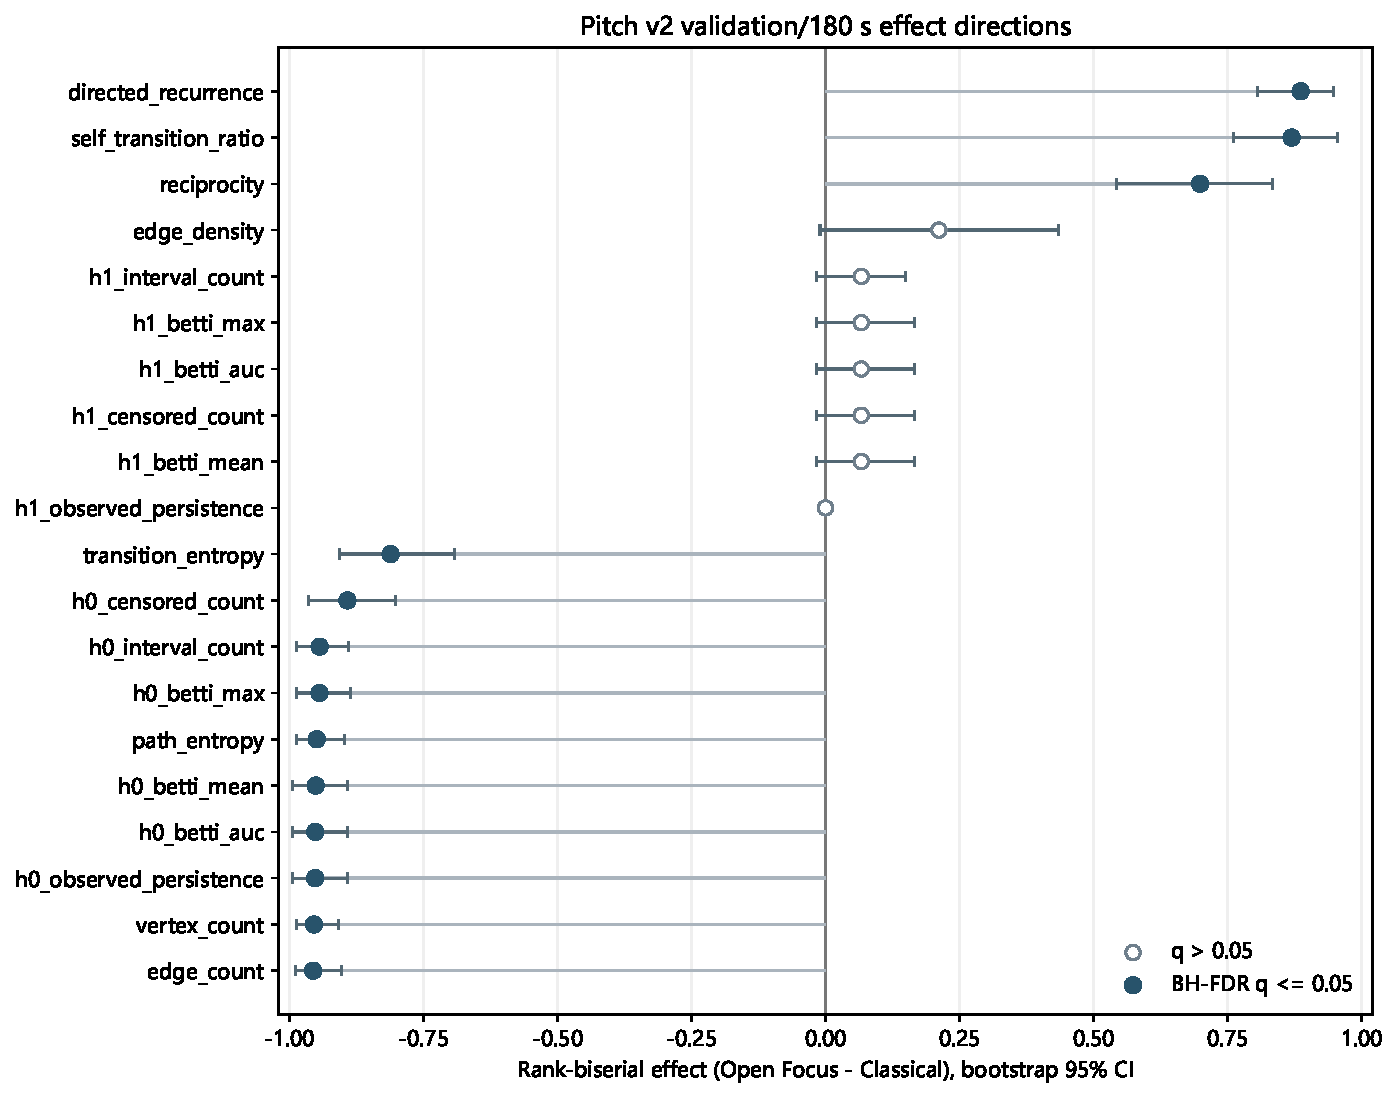
\includegraphics[width=\textwidth]{fig/pitch_v2_effect_sizes.pdf}
        \caption{Comparison of rank-biserial effect sizes for the pitch view}
        \label{fig:pitch_effect_size}
    \end{minipage}
    \hfill
    \begin{minipage}{0.46\textwidth}
        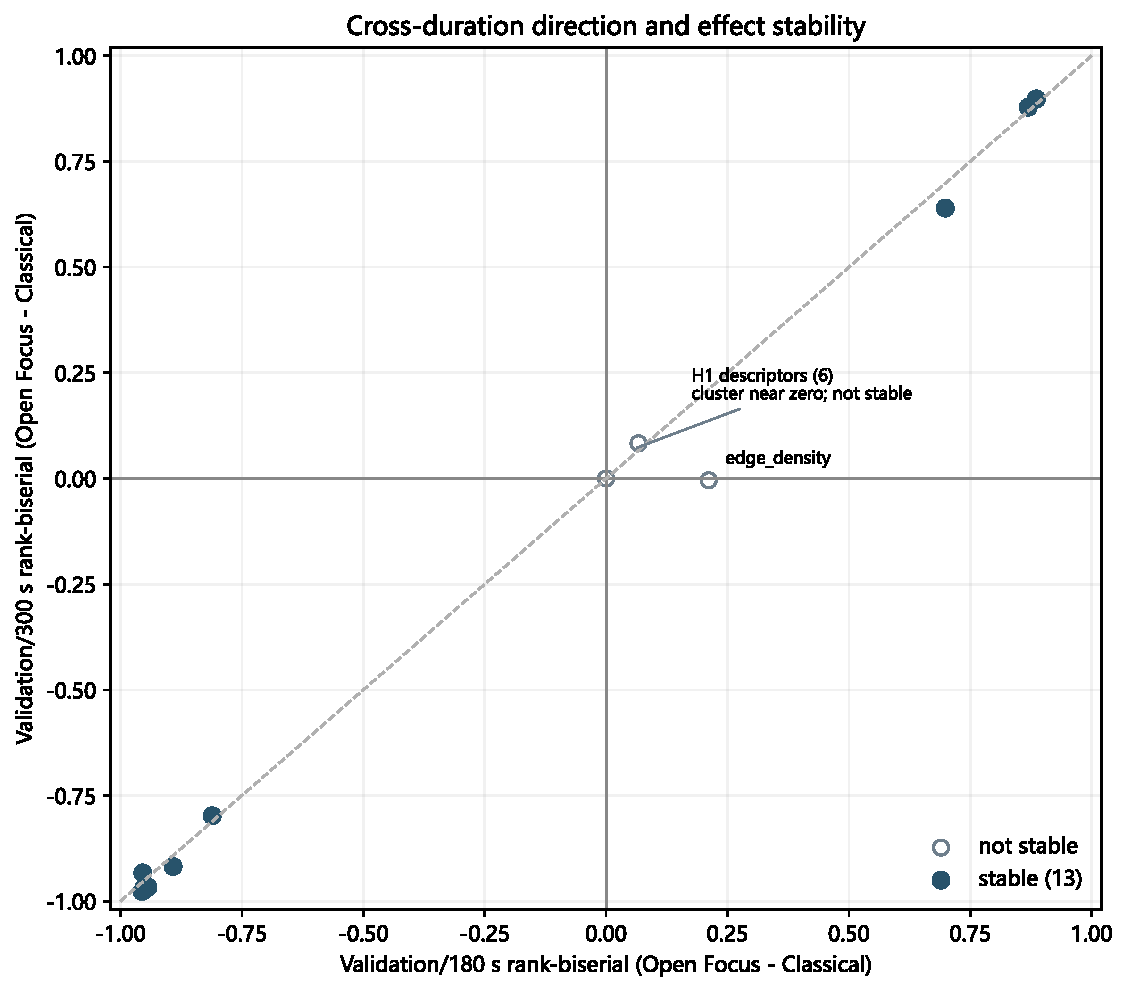
\includegraphics[width=\textwidth]{fig/pitch_v2_duration_stability.pdf}
        \caption{Cross-duration stability of the pitch view}
        \label{fig:pitch_duration_stability}
    \end{minipage}
\end{figure}

\begin{figure}[htbp]
    \centering
    \begin{minipage}{0.5\textwidth}
        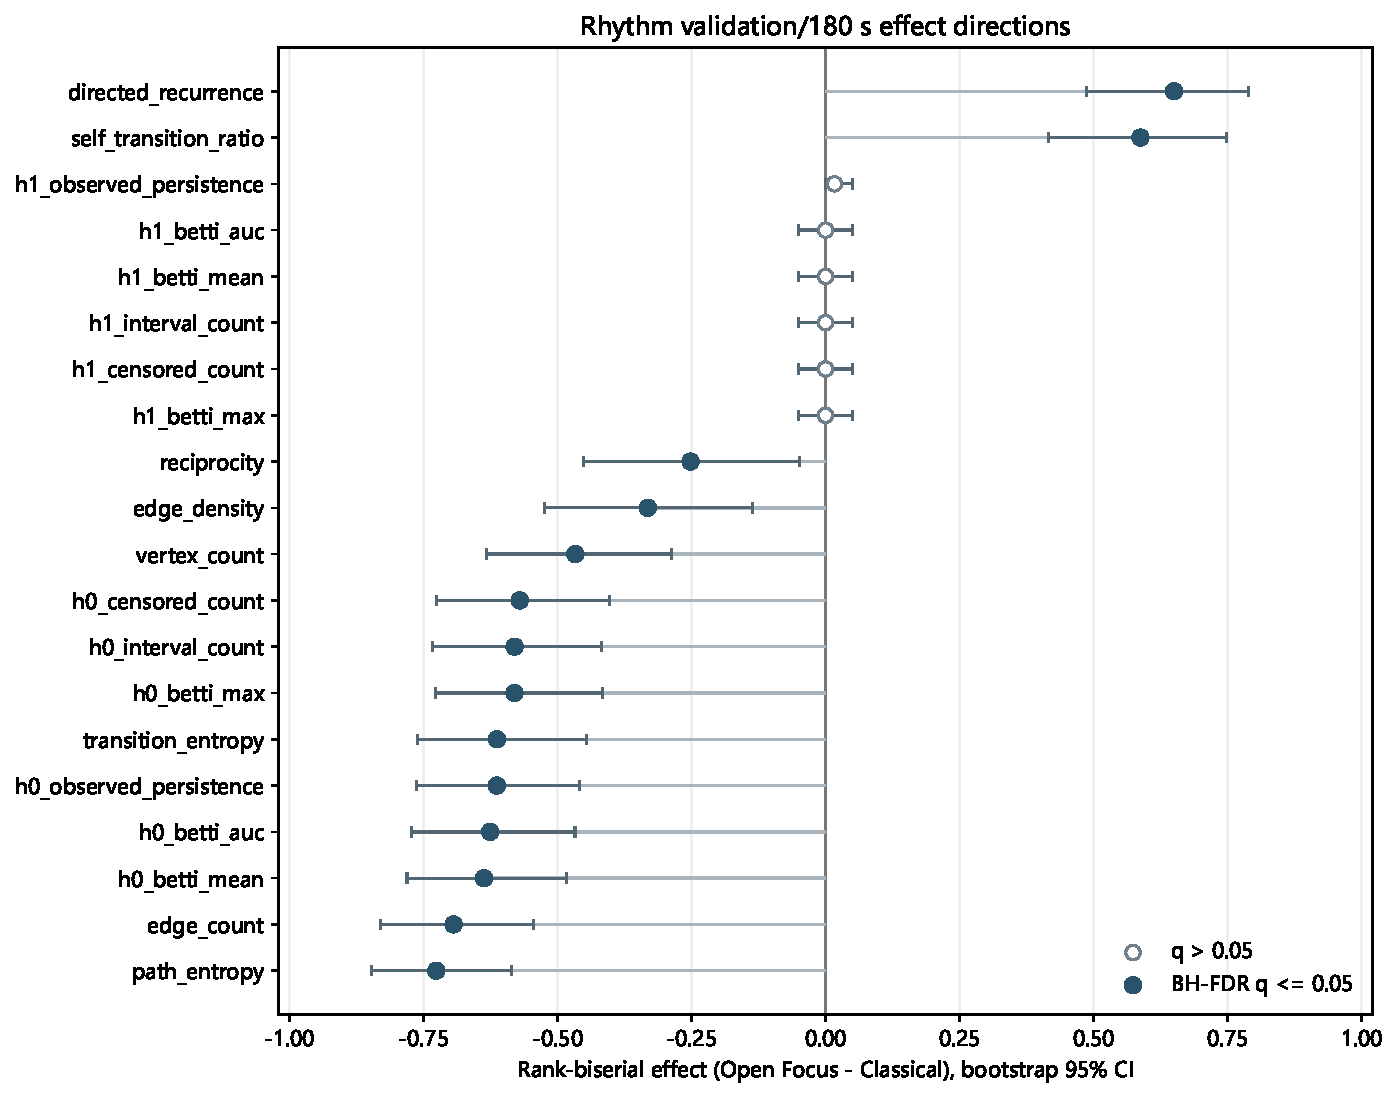
\includegraphics[width=\textwidth]{fig/rhythm_effect_sizes.pdf}
        \caption{Comparison of rank-biserial effect sizes for the rhythm view}
        \label{fig:rhythm_effect_size}
    \end{minipage}
    \hfill
    \begin{minipage}{0.46\textwidth}
        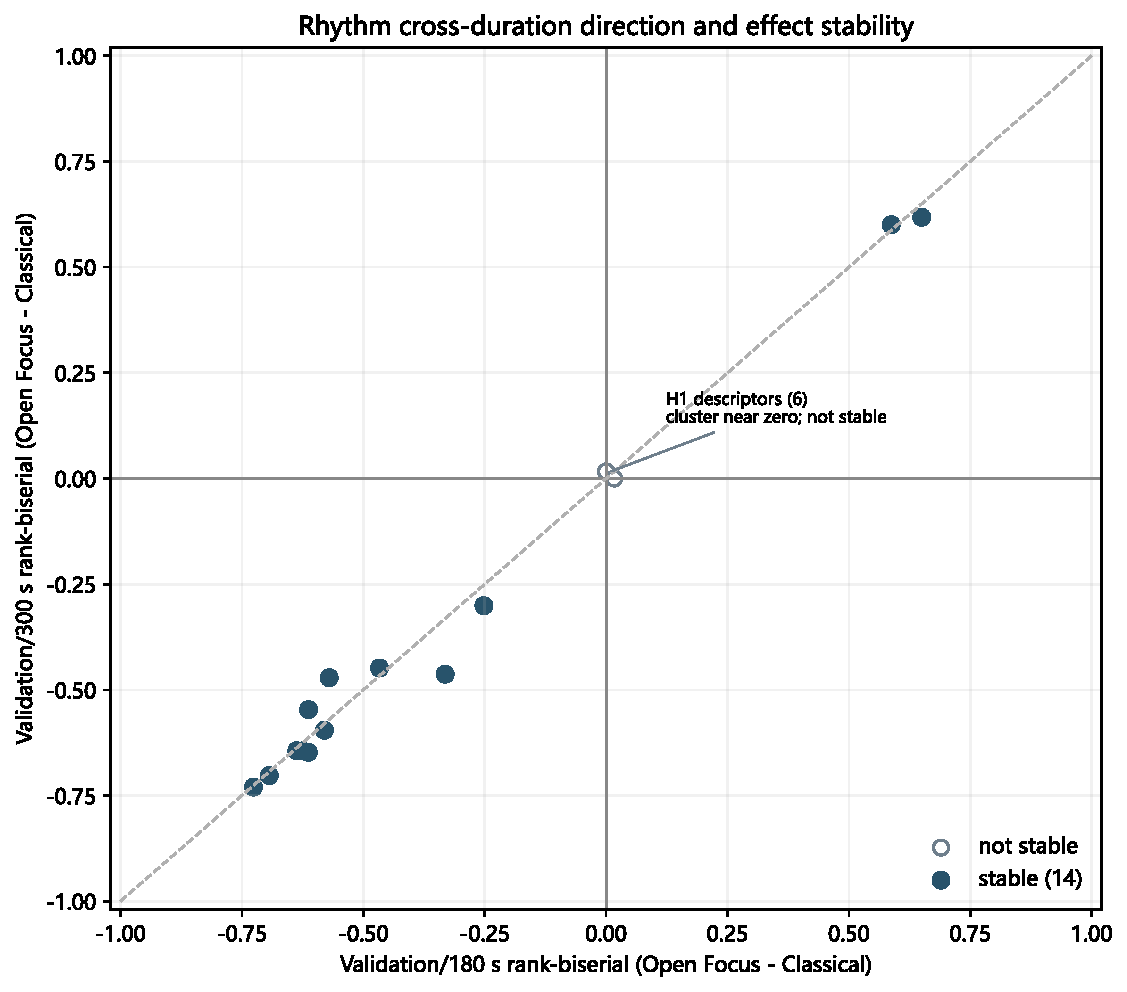
\includegraphics[width=\textwidth]{fig/rhythm_duration_stability.pdf}
        \caption{Cross-duration stability of the rhythm view}
        \label{fig:rhythm_duration_stability}
    \end{minipage}
\end{figure}

\begin{figure}[htbp]
    \centering
    \begin{minipage}{0.5\textwidth}
        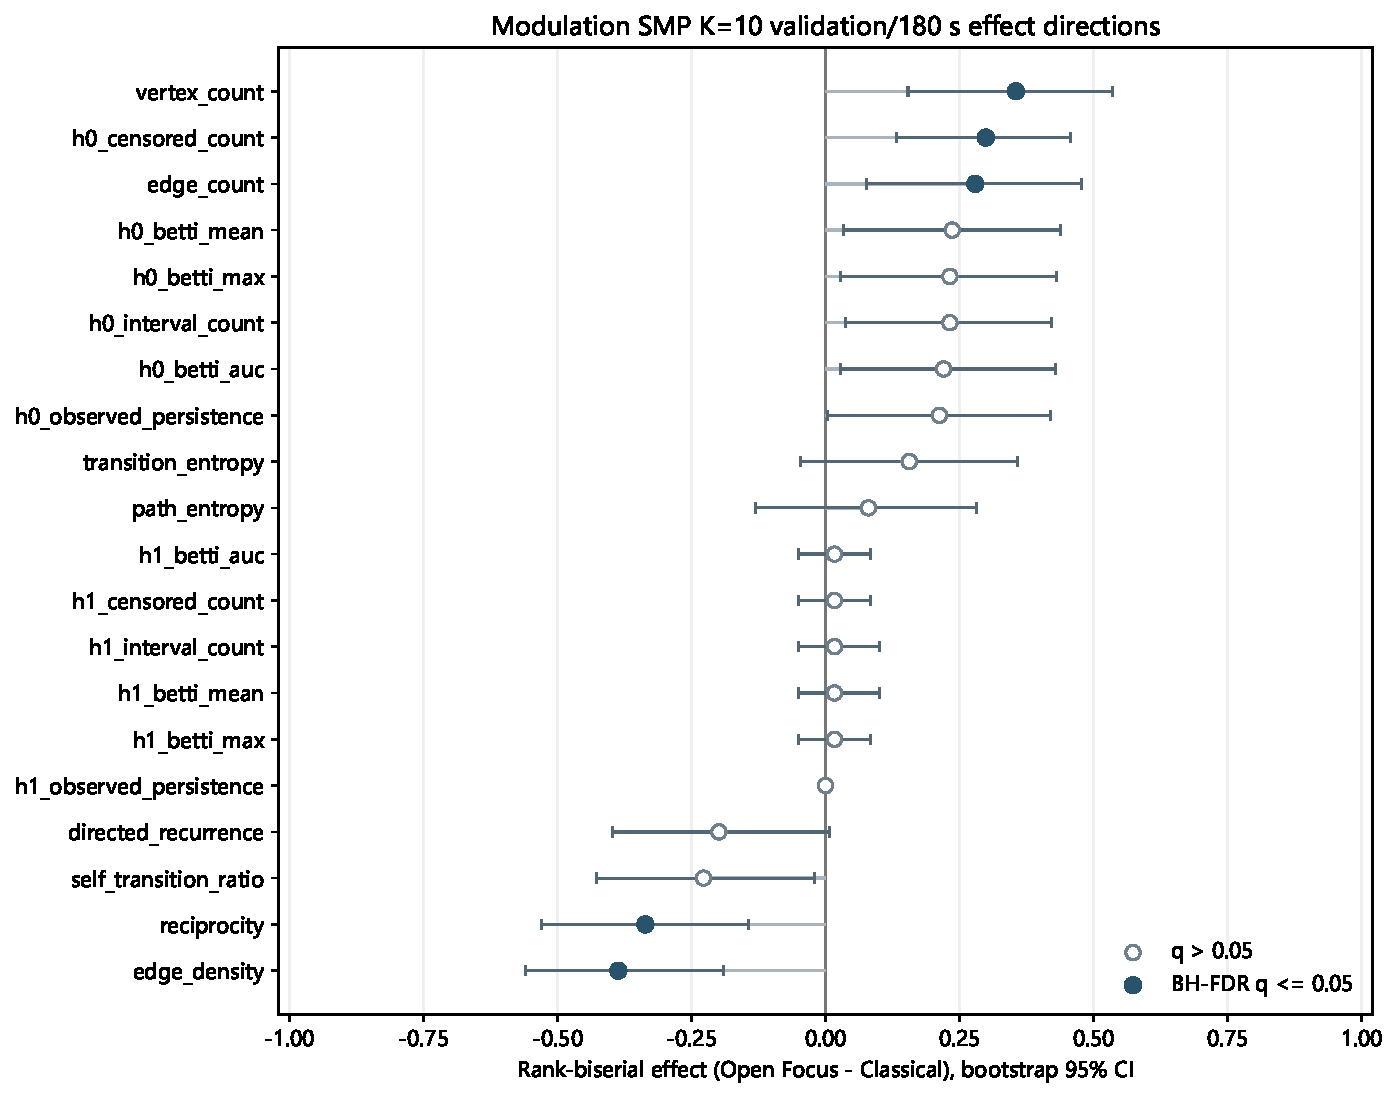
\includegraphics[width=\textwidth]{fig/modulation_smp_effect_sizes.pdf}
        \caption{Comparison of rank-biserial effect sizes for the modulation view}
        \label{fig:modulation_effect_size}
    \end{minipage}
    \hfill
    \begin{minipage}{0.46\textwidth}
        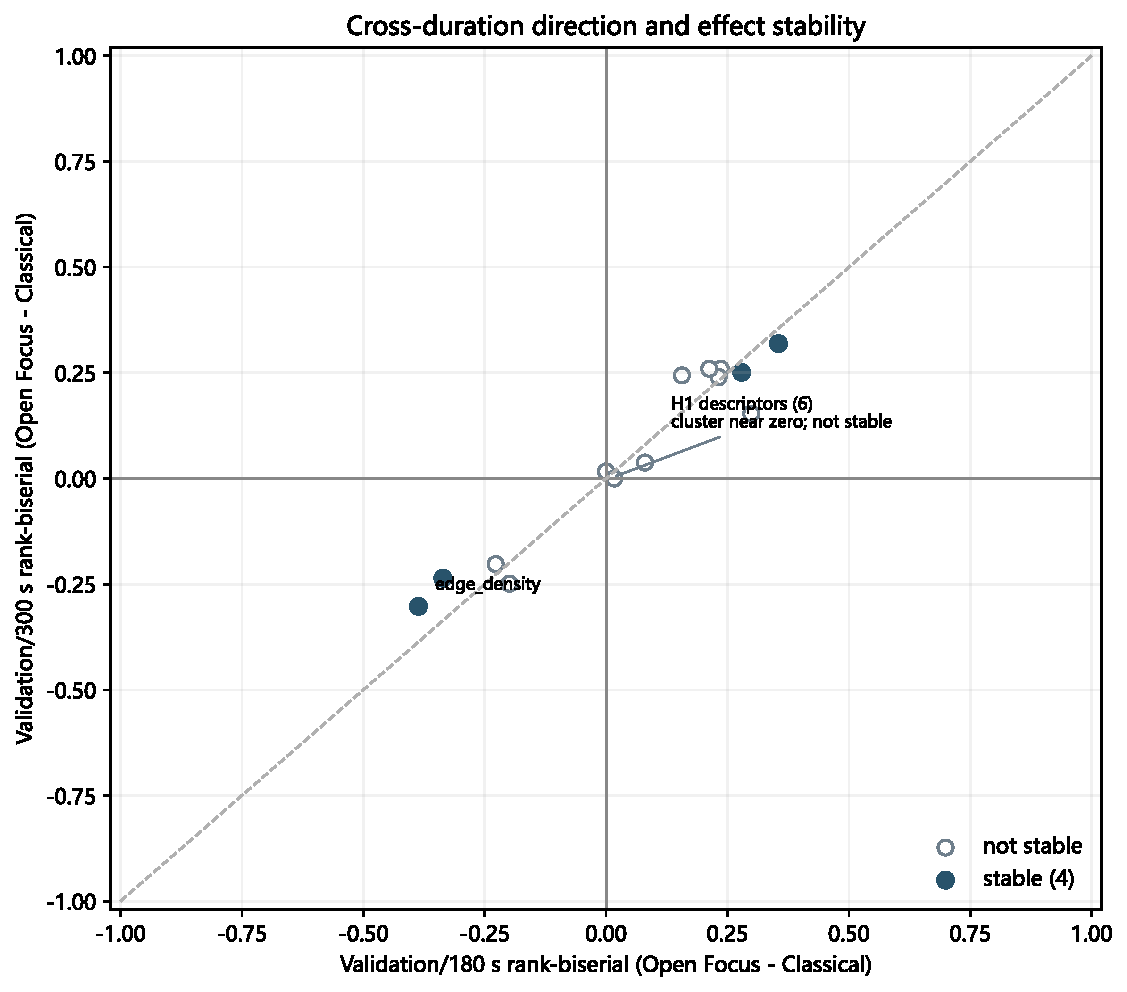
\includegraphics[width=\textwidth]{fig/modulation_smp_duration_stability.pdf}
        \caption{Cross-duration stability of the modulation view}
        \label{fig:modulation_duration_stability}
    \end{minipage}
\end{figure}

The pitch and rhythm views exhibit a common organizational pattern: Classical generally occupies more local prototypes, forms more directed edges, and has higher path entropy and transition entropy; Open Focus exhibits a higher self-transition ratio and directed recurrence rate. In the pitch view, the median numbers of states and edges are $16$ versus $10$ and $70$ versus $31$ for Classical and Open Focus, respectively; the corresponding values in the rhythm view are $8$ versus $7$ and $36$ versus $21$. Meanwhile, the pitch self-transition ratio and directed recurrence rate of Open Focus are $0.631$ and $0.114$, higher than the $0.322$ and $0.025$ of Classical; the corresponding values in the rhythm view are $0.662$, $0.265$ versus $0.479$, $0.092$. Therefore, the common difference between the two groups can be summarized as follows: Classical has broader state coverage and transition diversity, whereas the local state paths of Open Focus are more concentrated and more repetitive.

This commonality cannot be extrapolated to all connectivity metrics. Pitch reciprocity is higher in Open Focus ($0.667$ versus $0.522$), suggesting stronger bidirectional return between adjacent pitches; rhythm reciprocity, by contrast, is slightly higher in Classical ($0.809$ versus $0.769$), whose edge density is also higher. Therefore, ``Open Focus has stronger local recurrence'' refers only to the repetition of self-transitions and existing directed paths, and cannot be restated as the network being denser or more bidirectional across all views.

\begin{figure}[htbp]
    \centering
    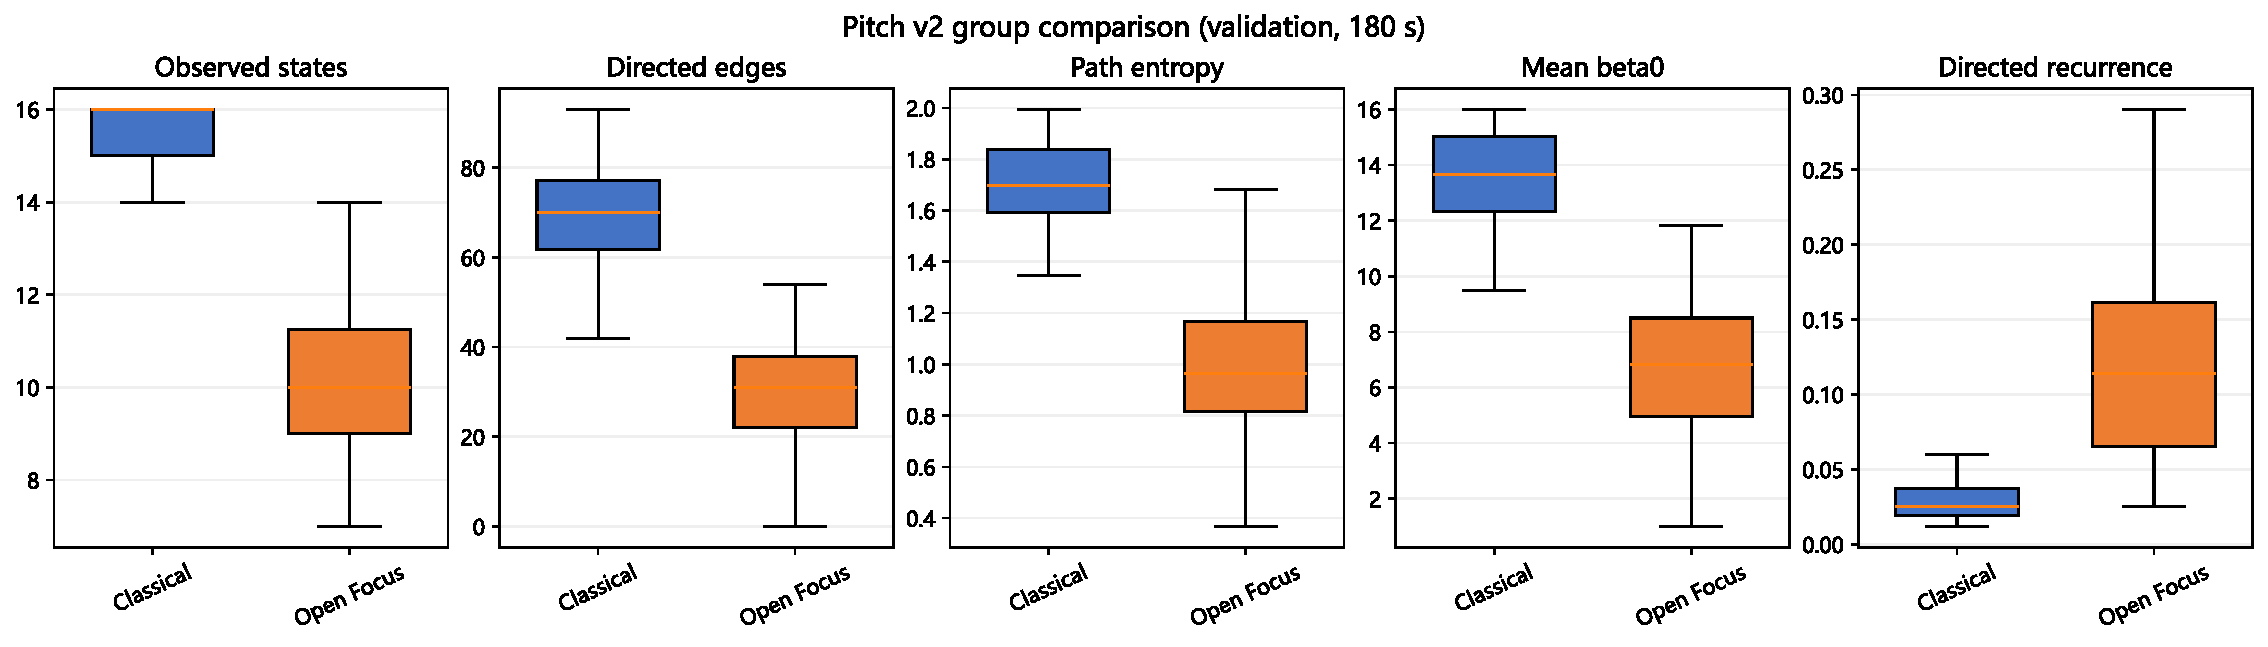
\includegraphics[width=\textwidth]{fig/pitch_v2_group_summary.pdf}
    \caption{Distributions of the main topological features of Classical and Open Focus in the pitch view.}
    \label{fig:pitch_group_summary}
\end{figure}

\begin{figure}[htbp]
    \centering
    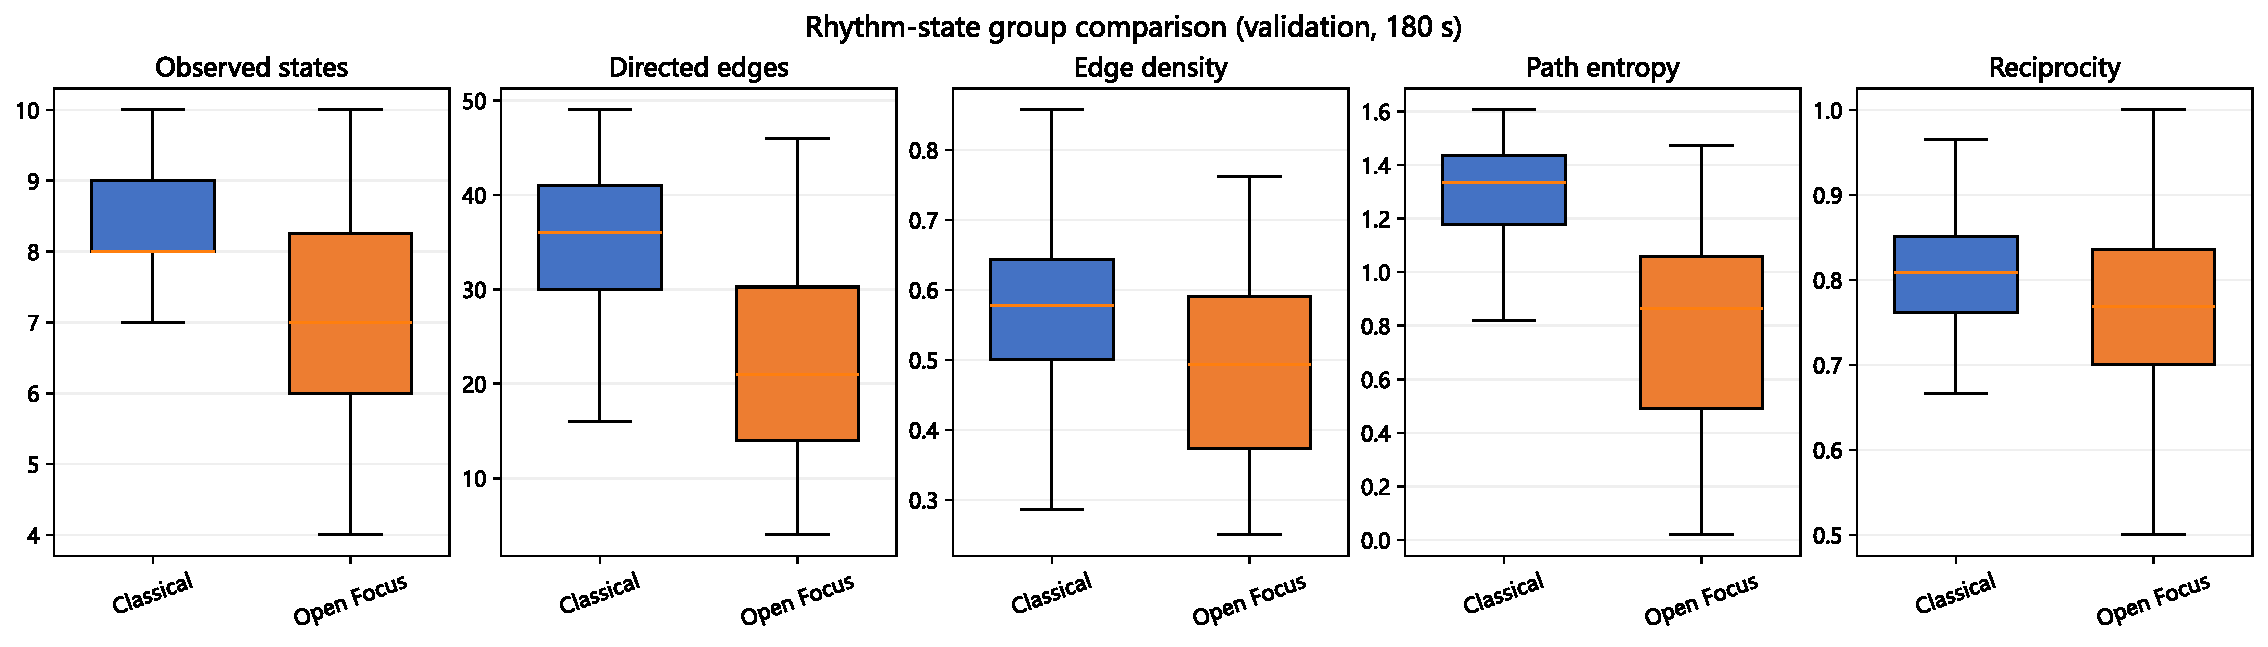
\includegraphics[width=\textwidth]{fig/rhythm_group_summary.pdf}
    \caption{Distributions of the main topological features of Classical and Open Focus in the rhythm view.}
    \label{fig:rhythm_group_summary}
\end{figure}

\begin{figure}[htbp]
    \centering
    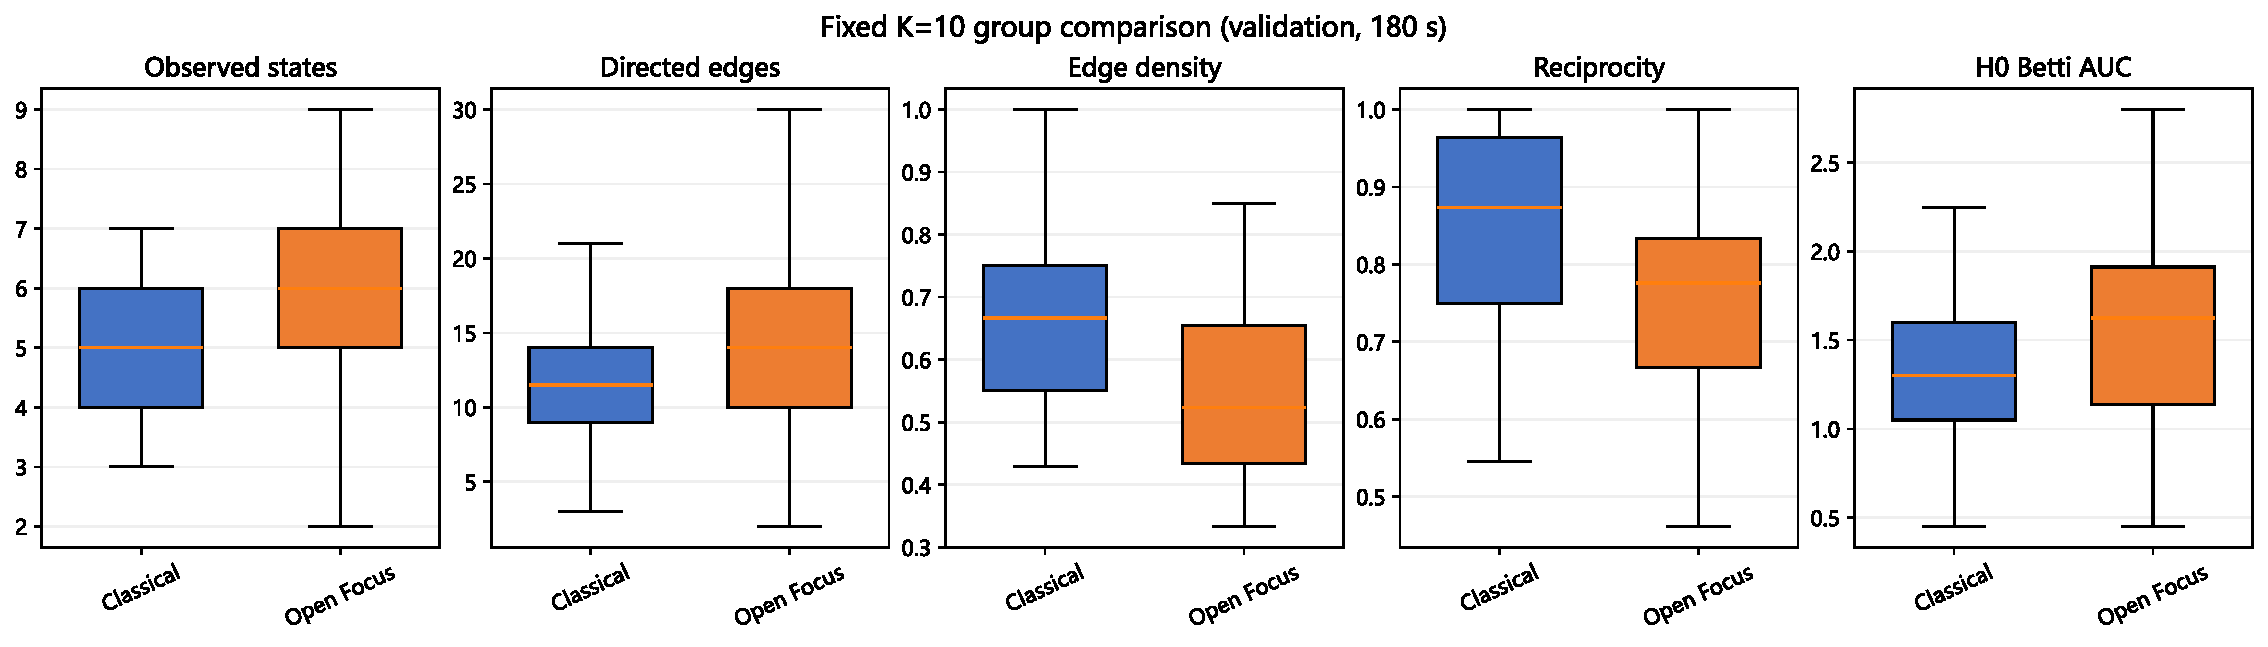
\includegraphics[width=\textwidth]{fig/modulation_smp_k10_group_summary.pdf}
    \caption{Distributions of the main topological features of Classical and Open Focus in the modulation view.}
    \label{fig:modulation_group_summary}
\end{figure}

The modulation view exhibits a pattern different from pitch and rhythm. In the shared $10$-state SMP codebook, Open Focus visits more prototypes and forms more absolute edges, with median state and edge counts of $6$ and $14$, higher than the $5$ and $11.5$ of Classical; however, its edge density and reciprocity are $0.524$ and $0.776$, lower than the $0.667$ and $0.873$ of Classical. This indicates that under the current SMP representation, Open Focus has broader coverage but sparser connections relative to the potential edge space and fewer bidirectional paired transitions. The $\epsilon^2$ of the four cross-duration stable metrics is $0.051$--$0.105$, and the absolute rank-biserial values are $0.279$--$0.386$; this result should therefore serve as an exploratory interpretation layer with limited effects, not as a confirmed core fingerprint.

The Betti curves of the three views are shown in Figures~\ref{fig:pitch_betti_curves}--\ref{fig:modulation_betti_curves}. At the homology level, the $H_0$ results for pitch and rhythm are consistent with the state coverage differences: Classical retains more connected components throughout the frozen filtration and undergoes more complete component merging. However, the $H_0$ descriptors are also affected by the number of actually occupied vertices and should be interpreted jointly with the state count, edge count, and entropy; they cannot be stated in isolation as one group having higher or better topological complexity. In the modulation view, only \verb|h0_censored_count| passes FDR at 180s, and it is no longer significant at 300s ($q=0.159$), so no stable $H_0$ conclusion is formed.

None of the three views supports a stable between-group $H_1$ difference. Within the primary threshold range, the numbers of segments with nonzero $H_1$ are 2/60 for Classical and 6/60 for Open Focus in the pitch view, 1/60 for both groups in the rhythm view, and 2/60 and 3/60 in the modulation view; the group medians of the six prespecified $H_1$ metrics are all 0, and no metric passes the 180s primary-analysis FDR. Therefore, the main discriminative information of the local views comes from state coverage, transition concentration, local recurrence, and the $H_0$ connectivity process, rather than from robust higher-order loop structures.

\begin{figure}[htbp]
    \centering
    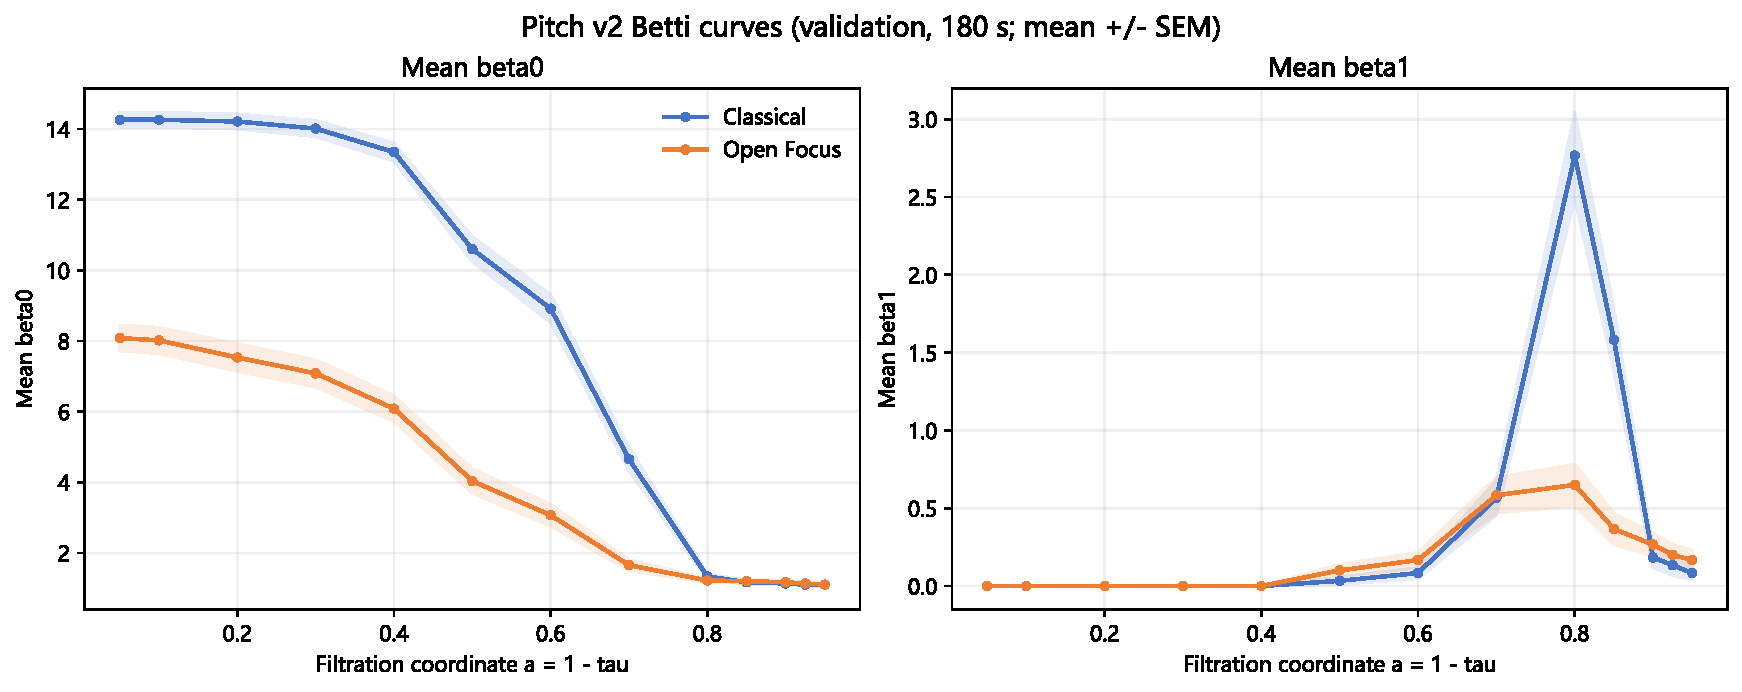
\includegraphics[width=\textwidth]{fig/pitch_v2_betti_curves.pdf}
    \caption{Betti curves of the pitch view.}
    \label{fig:pitch_betti_curves}
\end{figure}

\begin{figure}[htbp]
    \centering
    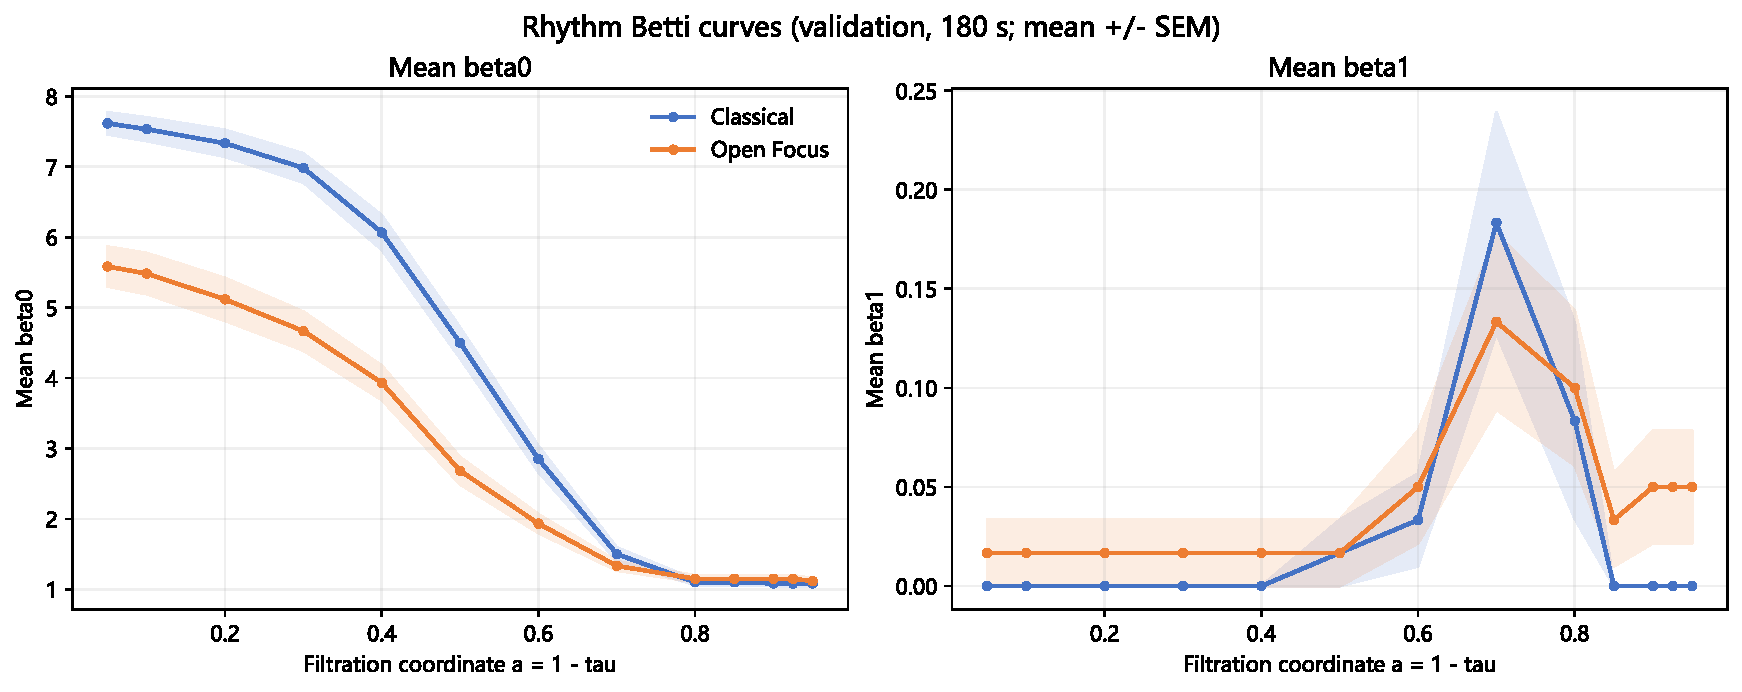
\includegraphics[width=\textwidth]{fig/rhythm_betti_curves.pdf}
    \caption{Betti curves of the rhythm view.}
    \label{fig:rhythm_betti_curves}
\end{figure}

\begin{figure}[htbp]
    \centering
    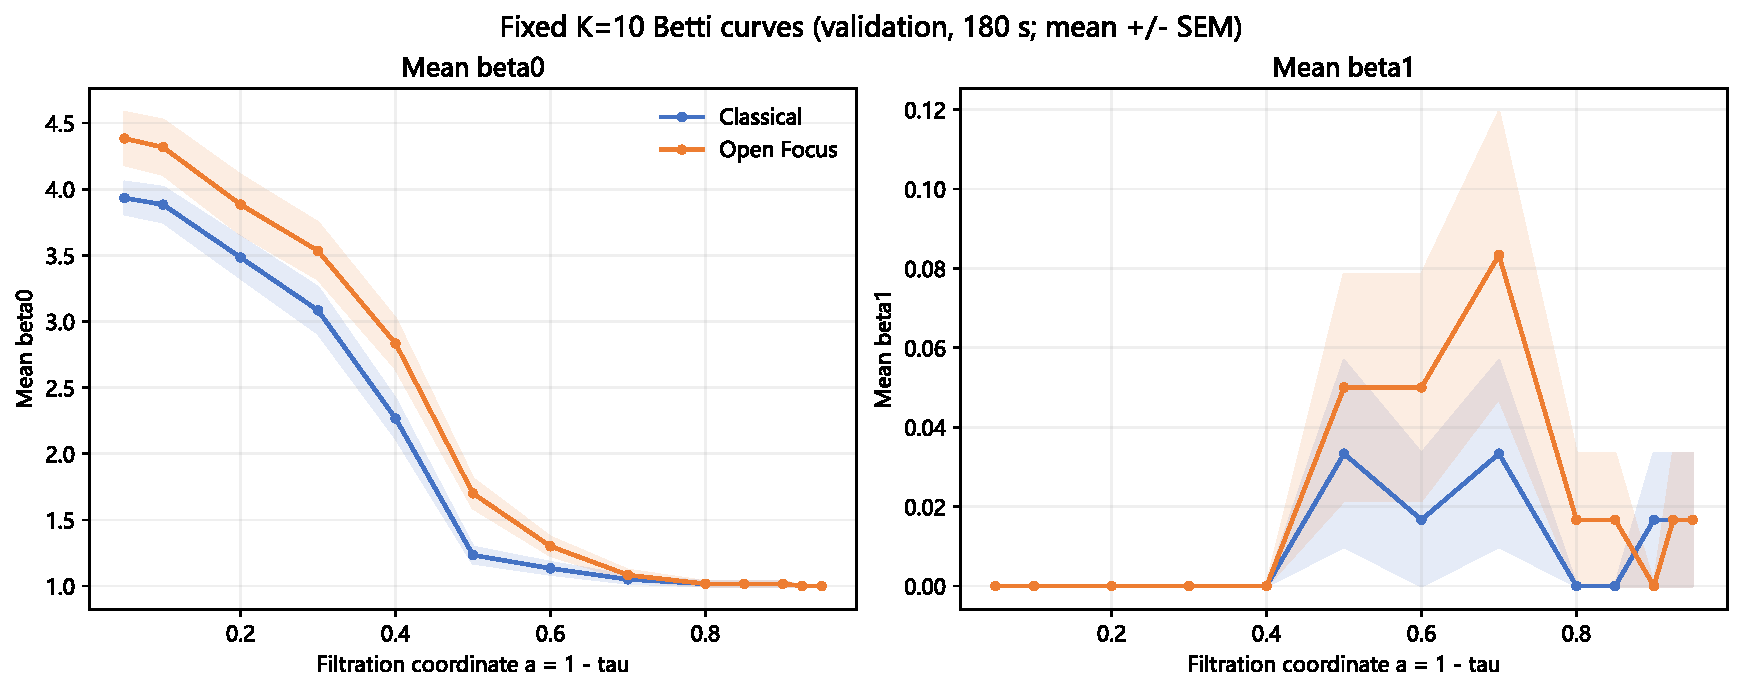
\includegraphics[width=\textwidth]{fig/modulation_smp_betti_curves.pdf}
    \caption{Betti curves of the modulation view.}
    \label{fig:modulation_betti_curves}
\end{figure}

\subsection{Multi-View Fusion and Ablation Analysis}
\label{sec:local_multiview_fusion}

The pitch, rhythm, and modulation describe respectively harmonic position, rhythmic organization, and amplitude modulation contour. To test whether this information can be complementary without constructing a high-dimensional Cartesian product state, this section performs late fusion of the three sets of 20 prespecified topological descriptors as independent blocks. The overall pipeline is shown in Figure~\ref{fig:local_multiview_fusion}.

\begin{figure}[htbp]
  \centering
  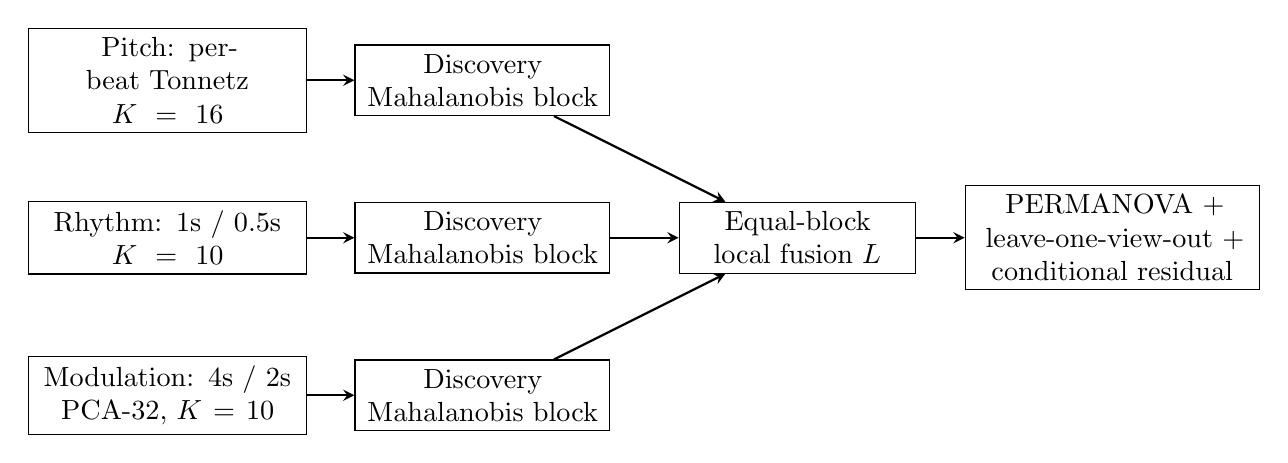
\begin{tikzpicture}[
      node distance=1.5cm,
      block/.style={rectangle, draw, minimum width=3cm, minimum height=0.8cm, text centered},
      arrow/.style={->, >=stealth, thick}
  ]
      % Input nodes
      \node[block, text width=3.3cm] (P) {Pitch: per-beat Tonnetz\\$K=16$};
      \node[block, text width=3.3cm, below of=P, yshift=-0.5cm] (R) {Rhythm: 1s / 0.5s\\$K=10$};
      \node[block, text width=3.3cm, below of=R, yshift=-0.5cm] (M) {Modulation: 4s / 2s\\PCA-32, $K=10$};

      % Mahalanobis blocks
      \node[block, text width=3cm, right of=P, xshift=2.5cm] (WP) {Discovery \\Mahalanobis block};
      \node[block, text width=3cm, right of=R, xshift=2.5cm] (WR) {Discovery \\Mahalanobis block};
      \node[block, text width=3cm, right of=M, xshift=2.5cm] (WM) {Discovery \\Mahalanobis block};

      % Fusion node
      \node[block, text width=2.5cm, right of=WR, xshift=2.5cm] (L) {Equal-block \\local fusion $L$};

      % Analysis node
      \node[block, text width=3.5cm, right of=L, xshift=2.5cm] (A) {PERMANOVA + leave-one-view-out + conditional residual};

      % Arrows
      \draw[arrow] (P) -- (WP);
      \draw[arrow] (R) -- (WR);
      \draw[arrow] (M) -- (WM);
      \draw[arrow] (WP) -- (L);
      \draw[arrow] (WR) -- (L);
      \draw[arrow] (WM) -- (L);
      \draw[arrow] (L) -- (A);
  \end{tikzpicture}
  \caption{Multi-view fusion analysis framework}
  \label{fig:local_multiview_fusion}
\end{figure}

\paragraph{Frozen block normalization and test design}
Direct concatenation would let views with higher effective dimensionality or larger covariance scale dominate the distances. For the discovery/180s descriptor matrix of view $v\in\{P,R,M\}$, missing values are first imputed with the discovery median, constant columns are removed, and the mean $\mu_v$ and covariance $\Sigma_v$ are then estimated. Letting $r_v$ denote its effective rank, the whitening matrix $W_v$ induced by the pseudoinverse of $\Sigma_v$ defines
\[
z_v(x)=\frac{(x-\mu_v)W_v}{\sqrt{r_v}},
\qquad W_vW_v^{\mathsf T}=\Sigma_v^{+}.
\]
The effective ranks of the pitch, rhythm, and modulation blocks are $13$, $13$, and $14$, respectively. After division by $\sqrt{r_v}$, the blocks have similar expected squared-distance scales; the equal-weight fusion of the three views and the combination of any two views are written as
\[
z_L(x)=\frac{1}{\sqrt{3}}[z_P(x)\Vert z_R(x)\Vert z_M(x)],
\qquad
z_{PR}(x)=\frac{1}{\sqrt{2}}[z_P(x)\Vert z_R(x)],
\]

The primary test is PERMANOVA based on Euclidean distance, with $999$ label permutations for each representation. The seven single-view or combined representations are BH-FDR corrected separately by duration. To determine whether a view genuinely adds between-group separation geometry, under the same label permutation we compute
\[
\Delta F=F^{*}_{\mathrm{candidate}}-F^{*}_{\mathrm{baseline}},
\]
and the six comparisons of ``full fusion relative to a single view'' and ``adding one view'' are corrected separately by duration; only $\Delta F>0$ with $q\leq0.05$ is counted as a positive increment. In addition, a multi-output ridge regression $\widehat f_v$ is fitted on discovery/180s using the other two blocks, and PERMANOVA is run again on the validation residuals
\[
R_v=Z_v-\widehat f_v(Z_{-v})
\]
to diagnose whether the target view contains group information that cannot be predicted from the other two views. This conditional residual test is not equivalent to a causal decomposition, nor does it guarantee that adding the view necessarily improves the overall distance discrimination.

\paragraph{Overall separation and combination ablation}
Table~\ref{tab:local_fusion_permanova} shows that all seven representations distinguish Open Focus from Classical at both durations (raw permutation $p$ all $0.001$, BH-FDR $q=0.001$). The pseudo-$F$ of the full fusion is $6.27$ at 180s and $10.54$ at 300s; however, the strongest single view at 180s is pitch ($F^{*}=7.59$), and at 300s it is also pitch ($F^{*}=18.19$). Therefore, the significance of the full fusion only shows that the fused space retains between-group differences; it cannot be used to claim that it outperforms the best single view.

\begin{table}[htbp]
\centering
\caption{PERMANOVA results of the local three-view fusion and combination ablation}
\label{tab:local_fusion_permanova}
\renewcommand{\arraystretch}{1.5}
\setlength{\tabcolsep}{12pt}
\begin{tabular}{lrrrrr}
\toprule
Representation & Dim & 180s $F^{*}$ & 180s $q$ & 300s $F^{*}$ & 300s $q$ \\
\midrule
Pitch ($P$) & 16 & 7.59 & 0.001 & 18.19 & 0.001 \\
Rhythm ($R$) & 16 & 6.47 & 0.001 & 10.24 & 0.001 \\
Modulation ($M$) & 17 & 4.13 & 0.001 & 4.24 & 0.001 \\
$P+R$ & 32 & 7.08 & 0.001 & 14.11 & 0.001 \\
$P+M$ & 33 & 6.17 & 0.001 & 10.69 & 0.001 \\
$R+M$ & 33 & 5.40 & 0.001 & 7.10 & 0.001 \\
$P+R+M$ & 49 & 6.27 & 0.001 & 10.54 & 0.001 \\
\bottomrule
\end{tabular}
\end{table}

\paragraph{Two-dimensional projection of the fusion space}
To visualize the sample relations in the full fusion representation, Figure~\ref{fig:local_fusion_pca} uses a PCA fitted only on discovery/180s to project the 49-dimensional fusion coordinates of validation/180s onto the first two principal components. Classical tracks are mainly distributed on the positive side of PC1 and are relatively concentrated, whereas Open Focus leans toward the negative side of PC1 as a whole and shows greater within-group dispersion, but the two groups still overlap considerably. PC1 and PC2 explain only $4.8\%$ and $4.7\%$ of the variance, respectively, totaling $9.5\%$; the figure therefore provides only low-dimensional geometric intuition and does not participate in PERMANOVA or paired incremental tests.

\begin{figure}[htbp]
    \centering
    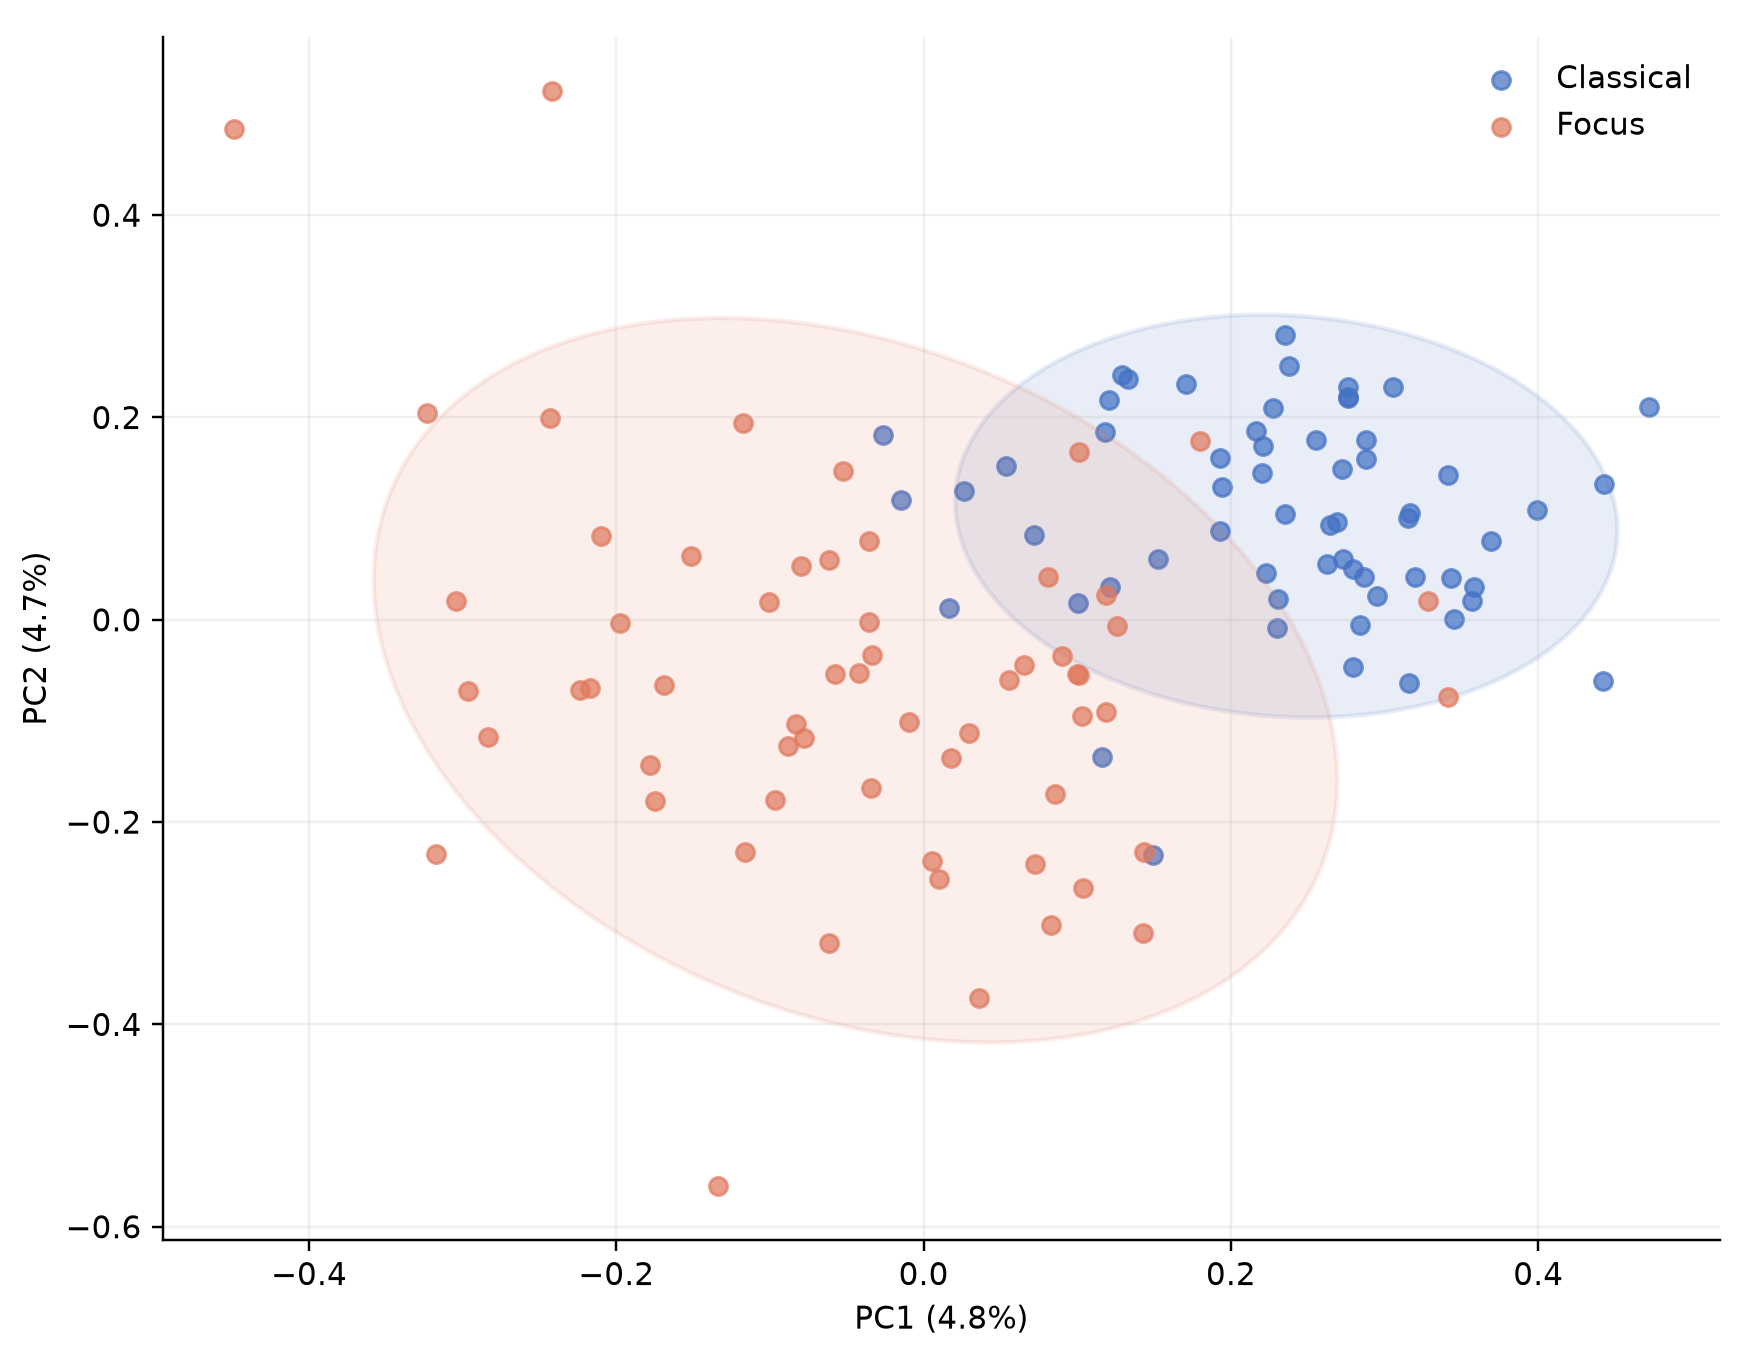
\includegraphics[width=0.78\textwidth]{fig/local_smp_k10_pca_validation_180.png}
    \caption{Two-dimensional projection of the validation/180s three-view fusion representation by a PCA fitted on discovery/180s. Each point represents one track; the elliptical shading indicates the projection range centered at the within-group mean and extending $1.96$ standard deviations along the principal axes of the within-group covariance, and is not a bootstrap confidence interval.}
    \label{fig:local_fusion_pca}
\end{figure}

\paragraph{Incremental gain and conditional non-redundancy}
The paired incremental results are shown in Figure~\ref{fig:local_fusion_incremental}. In the 180s primary analysis, the $\Delta F$ of the full fusion relative to pitch is $-1.32$ ($q=1$), and relative to rhythm it is $-0.205$ ($q=1$); relative to modulation it is $2.14$ ($q=0.003$), but this only shows that the fusion outperforms the weaker single view of modulation. In the leave-one-view-out ablation, adding pitch to ``rhythm + modulation'' yields a stable positive increment (180s: $\Delta F=0.864$, $q=0.003$; 300s: $3.44$, $q=0.003$). Adding rhythm to ``pitch + modulation'' yields an increment of only $0.101$ at 180s ($q=0.462$), and adding modulation to ``pitch + rhythm'' instead yields $-0.814$ ($q=1$); neither provides evidence of a positive increment. This result identifies pitch as the main separating block in the current equal-weight distance, and does not support the hypothesis that ``every added view strengthens the between-group geometry''.

\begin{table}[htbp]
\centering
\caption{Paired pseudo-$F$ incremental test results of the local three-view fusion}
\label{tab:local_fusion_incremental}
\renewcommand{\arraystretch}{1.5}
\setlength{\tabcolsep}{12pt}
\begin{tabular}{lrrrr}
\toprule
Comparison & 180s $\Delta F$ & 180s FDR & 300s $\Delta F$ & 300s FDR \\
\midrule
Full-Pitch & -1.32 & 1 & -7.65 & 1 \\
Full-Rhythm & -0.205 & 1 & 0.298 & 0.342 \\
Full-Modulation & 2.14 & 0.003 & 6.3 & 0.003 \\
Add Pitch to Rhythm+Modulation & 0.864 & 0.003 & 3.44 & 0.003 \\
Add Rhythm to Pitch+Modulation & 0.101 & 0.462 & -0.146 & 1 \\
Add Modulation to Pitch+Rhythm & -0.814 & 1 & -3.56 & 1 \\
\bottomrule
\end{tabular}
\end{table}

\begin{figure}[htbp]
    \centering
    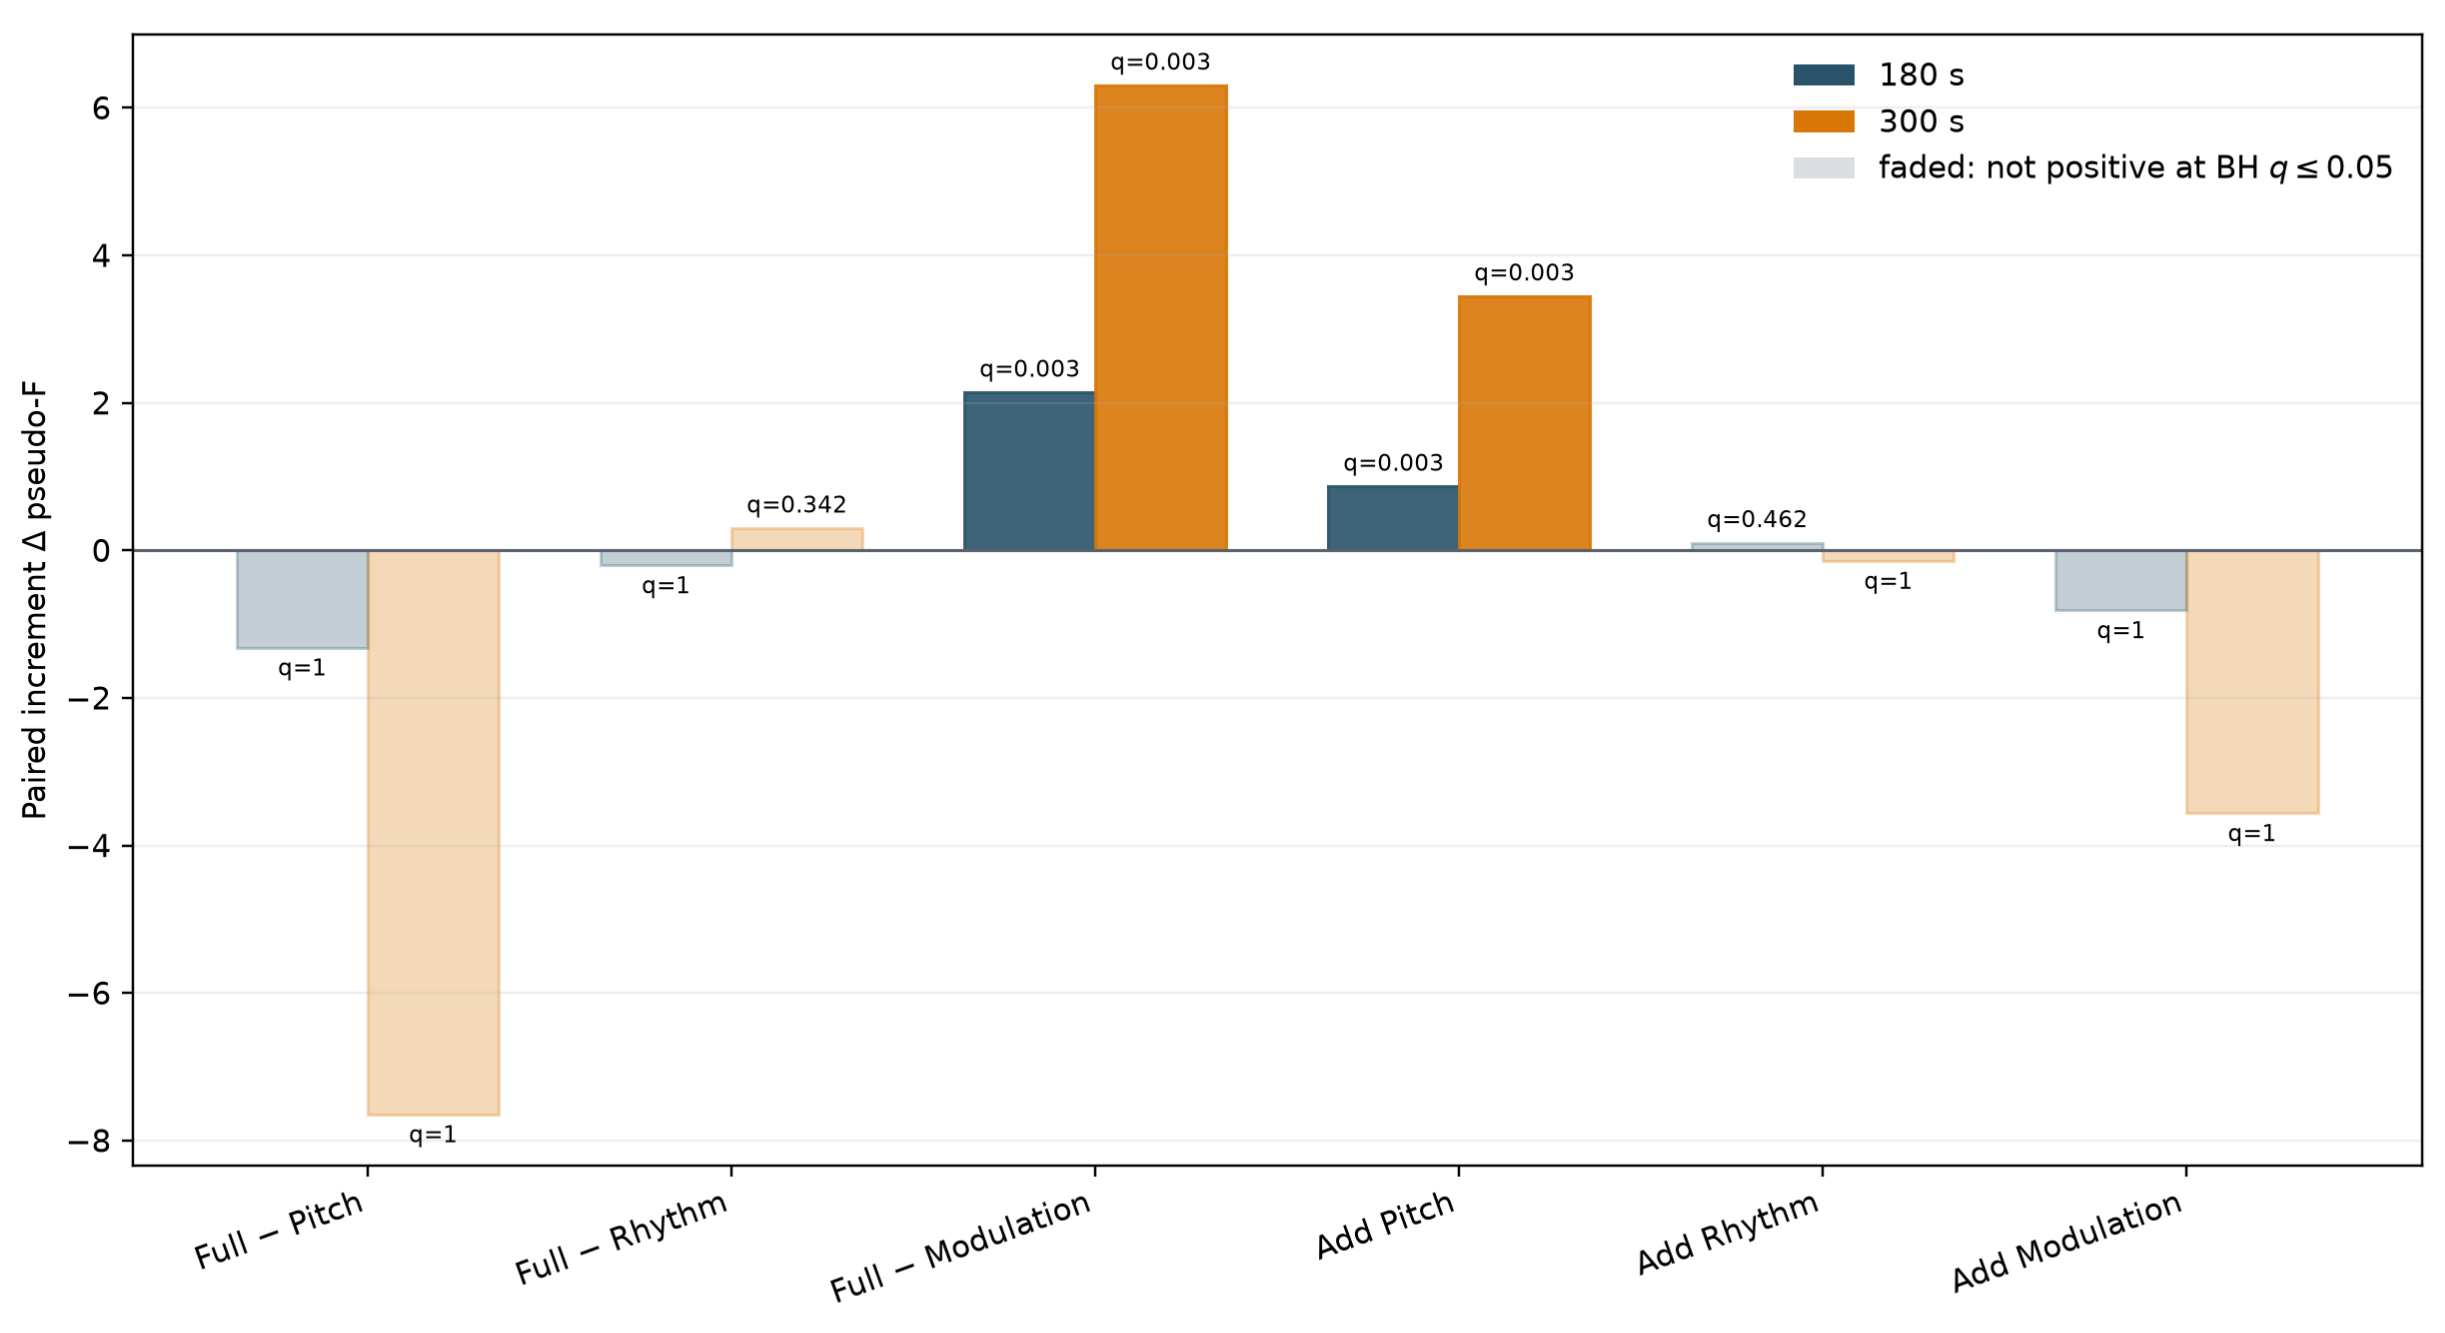
\includegraphics[width=\textwidth]{fig/local_smp_k10_incremental_tests.png}
    \caption{Paired pseudo-$F$ incremental tests of the local three-view fusion. Light-colored bars indicate that $\Delta F>0$ and BH-FDR $q\leq0.05$ are not both satisfied; 300s serves only as same-track duration sensitivity.}
    \label{fig:local_fusion_incremental}
\end{figure}

The conditional residuals answer a different but complementary question. In Table~\ref{tab:local_fusion_residual}, the residuals of all three views still contain significant group structure at 180s; the directions at 300s are also consistent. However, the validation $R^2$ of rhythm and modulation is close to zero or negative, indicating that the cross-view predictive relations fitted on discovery do not generalize stably. These results therefore support that the three views contain conditionally non-redundant information, but cannot be taken to imply that every view produces a verifiable positive increment to the equal-weight fusion.

\begin{table}[htbp]
\centering
\caption{Residual PERMANOVA of each local view conditioned on the other two views}
\label{tab:local_fusion_residual}
\renewcommand{\arraystretch}{1.5}
\setlength{\tabcolsep}{12pt}
\begin{tabular}{lrrrrr}
\toprule
Target view & 180s $F^{*}$ & 180s $q$ & validation $R^2$ & 300s $F^{*}$ & 300s $q$ \\
\midrule
Pitch & 4.53 & 0.0015 & 0.0476 & 11.74 & 0.0015 \\
Rhythm & 3.39 & 0.0015 & $-0.0089$ & 6.34 & 0.0015 \\
Modulation & 2.22 & 0.0100 & 0.0034 & 1.88 & 0.0310 \\
\bottomrule
\end{tabular}
\end{table}

\paragraph{Auxiliary classification and metric divergence}
As an auxiliary analysis, an L2 logistic regression with $C$ selected by five-fold cross-validation within discovery/180s is frozen and then applied to validation; classification differences use a within-group stratified bootstrap with $1{,}000$ resamples and a fixed seed. At 180s, the balanced accuracy, Macro-F1, and AUROC of the full fusion are $0.967$, $0.967$, and $0.991$, and those of the pitch single view are $0.925$, $0.925$, and $0.986$. The balanced accuracy increment of the full fusion over pitch is $0.0417$, with a bootstrap 95\% CI of $[0.0165,0.0750]$. In addition, adding modulation to $P+R$ increases the balanced accuracy by $0.0333$, with a 95\% CI of $[0.0083,0.0667]$; however, its distance increment is $\Delta F=-0.814$ with $q=1$. Classification performance measures per-track discrimination, whereas pseudo-$F$ measures the ratio of between-group distance to within-group dispersion, and the two can move in different directions; they must therefore be reported side by side, and only favorable metrics must not be selected.

\begin{figure}[htbp]
    \centering
    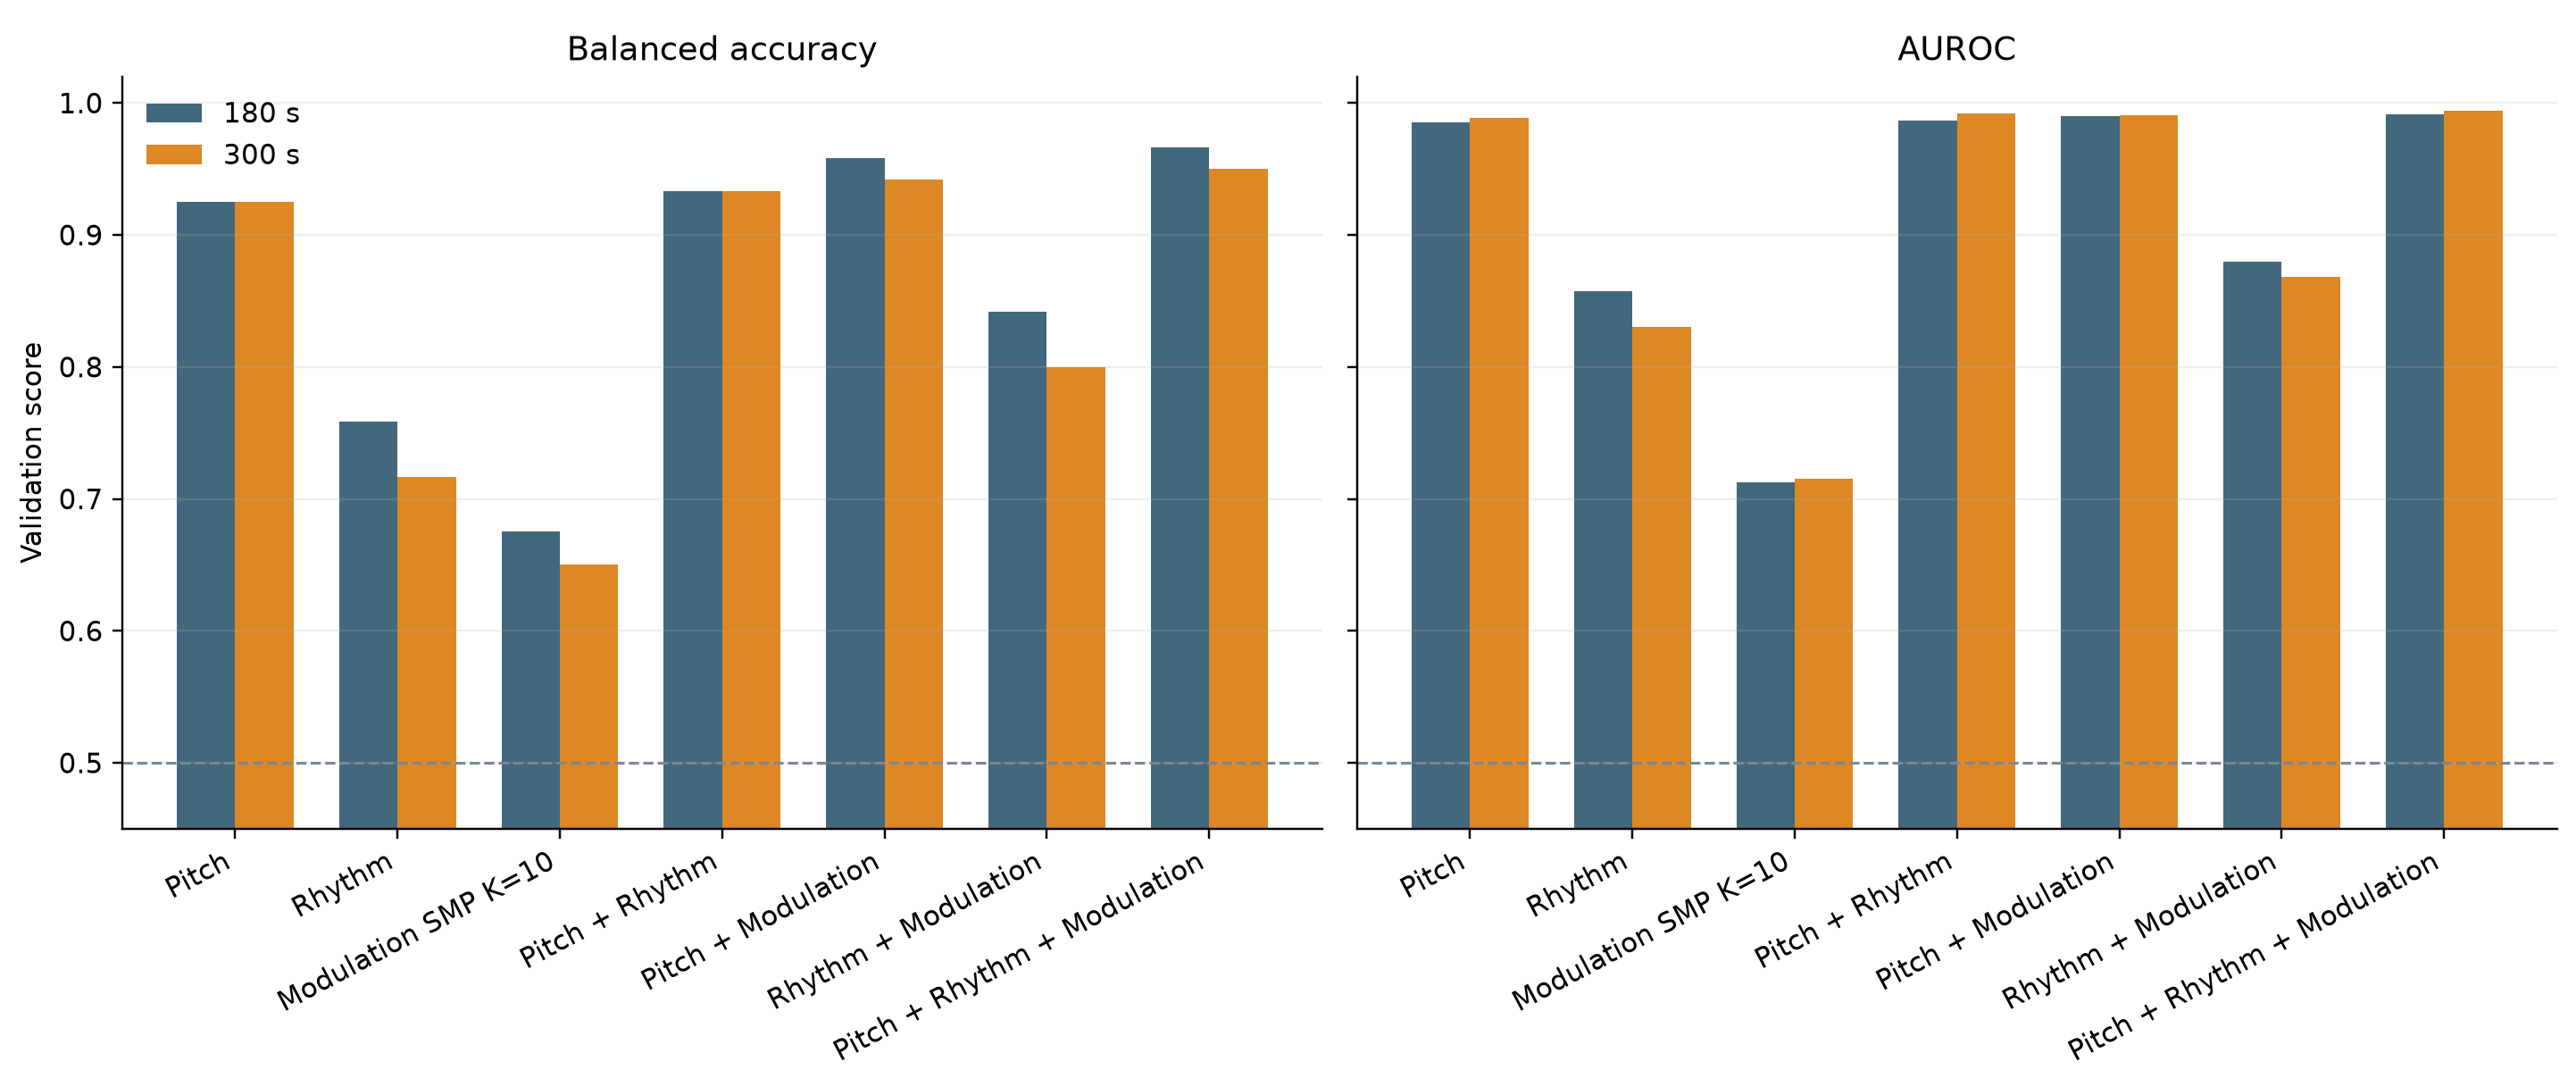
\includegraphics[width=\textwidth]{fig/local_smp_k10_classification_ablation.png}
    \caption{Auxiliary classification ablation results frozen on discovery/180s. The classification results supplement the distance-geometry tests and do not replace PERMANOVA or the paired incremental tests.}
    \label{fig:local_fusion_classification}
\end{figure}

\paragraph{Overall judgment and evidence boundaries}
The equal-weight fusion of the three local views retains stable between-group separability and outperforms the pitch single view in auxiliary per-track classification; however, it does not improve the pseudo-$F$ relative to the best single view, and the leave-one-view-out tests confirm a positive geometric increment only for pitch. Rhythm and modulation have conditional non-redundancy and independent explanatory value, but there is no evidence that they provide stable incremental separation in the current equal-weight distance. Therefore, \textbf{this paper regards pitch as the main separating block of the local fingerprint and retains rhythm and modulation as complementary interpretation blocks, without claiming that the three-view fusion is overall superior to the best single view}.

\subsection{Topological Fingerprint Freezing}
\label{sec:frozen_topology_fingerprint}

Based on the preceding single-view validation and multi-scale incremental analysis, this paper freezes the current Focus Music Path Homology fingerprint as an $18$-dimensional joint representation, denoted $\Phi_{\mathrm{PH}}$. The fingerprint contains only three inputs: Pitch local state transitions, the Acoustic phase closed loop, and the Chroma phase closed loop, and it can be expressed as:
\[\Phi_{\mathrm{PH}}=\frac{1}{\sqrt{2}}[L\Vert P]\]
where $L=Z_{\mathrm{Pitch}}$ and $P=\frac{1}{\sqrt{2}}
[Z_{\mathrm{Acoustic}}\Vert Z_{\mathrm{Chroma}}]$.

Table~\ref{tab:frozen_fingerprint} gives the frozen fields that constitute the identity of the current version.

\begin{table}[htbp]
\centering
\caption{Frozen composition of the Focus Music Path Homology topological fingerprint}
\label{tab:frozen_fingerprint}
\renewcommand{\arraystretch}{1.5}
\setlength{\tabcolsep}{8pt}
\begin{tabular}{lrrr}
\toprule
Input block & Output dim & Effective rank & Squared-distance weight \\
\midrule
Pitch Path Homology & 16 & 13 & $1/2$ \\
Acoustic phase \texttt{loop\_score} & 1 & 1 & $1/4$ \\
Chroma phase \texttt{loop\_score} & 1 & 1 & $1/4$ \\
\midrule
Joint fingerprint $\Phi_{\mathrm{PH}}$ & 18 & -- & 1 \\
\bottomrule
\end{tabular}
\end{table}

In addition to the composition and weights in Table~\ref{tab:frozen_fingerprint}, the following settings are frozen as well:
\begin{enumerate}
  \item 180s is the primary scale; the state codebooks, missing-value imputation, block transformations, and classifiers are fitted only on
  discovery, and validation/180s is used only for the primary evaluation;
  \item Pitch uses the frozen state representation and $20$ prespecified descriptors, retaining $16$ dimensions after the discovery
  constant columns are removed; the phase lifting is fixed at six phase nodes, and the \texttt{loop\_score} of Acoustic and
  Chroma is extracted respectively;
  \item the distance geometry uses PERMANOVA with $999$ permutations and bidirectional paired pseudo-$F$ increments,
  with BH-FDR within the prespecified test families; the conditional residual models are fitted only on discovery;
  \item the auxiliary L2 logistic regression selects its regularization parameter only by five-fold cross-validation within discovery, and the
  frozen parameter of the current joint representation is $C=10$; classification differences use $1{,}000$ within-group stratified paired bootstrap resamples;
  \item 300s serves only as same-track duration sensitivity; the already opened holdout is not used for parameter tuning, phase screening,
  weight changes, or generating new significance claims.
\end{enumerate}

The frozen object is an auditable scientific representation and evaluation protocol, not a causal scale of attention, efficacy, or musical quality. The logits or probabilities of the auxiliary classifier only describe the decision boundary in the current Open Focus--Classical data and do not change the $18$-dimensional definition of $\Phi_{\mathrm{PH}}$ itself.

After freezing, it is not allowed to change the $\frac{1}{2}:\frac{1}{4}:\frac{1}{4}$ weights, optimize the number of phase nodes, or select a new subset of metrics. Any such change should establish a new fingerprint version and redo the incremental, classification, and generation experiment validation on data that did not participate in that selection.

\section{ACE-Step Topology-Guided Music Generation}

One purpose of this paper is to apply the topological features of Focus Music to music generation. The traditional route would train a new music generation model and embed the topological features as a loss function in the training loop. However, training a high-quality music generation model requires large amounts of copyright-sensitive audio data and is demanding in GPU compute. This study therefore shifts the engineering core from ``updating the model parameters $\theta$'' to ``controlling the inference-time latent variables $z_t$''.

This study adopts ACE-Step 1.5 XL-Turbo as the base backbone and applies topological energy gradients derived from the frozen Path Homology fingerprint to the current audio latent variables at the key time steps of its reverse diffusion sampling. This preserves the music generation ability of the pretrained model while subjecting the generation process to an interpretable algebraic-topology constraint.

\subsection{Methodology and Overall Framework}

Because exact Path Homology (exact PH) involves a series of non-smooth operations whose gradients are zero or undefined almost everywhere, valid gradients cannot be propagated through the chain rule. We therefore train a Latent Topology Surrogate Network (LTSN) to provide approximate, differentiable scores from which gradients can be backpropagated. Its learning objective is to mimic the output of exact PH while keeping the entire computation graph differentiable.

The core of the whole method is an ``exact teacher, differentiable surrogate, exact re-verification'' closed loop:
exact PH is responsible for constructing training labels, performing same-prompt candidate reranking, and adjudicating the final audio; the LTSN only learns a differentiable approximation from the intermediate predicted clean latent variables to the frozen fingerprint; the sampler applies magnitude-limited mid-segment corrections only after the LTSN passes the independent qualification tests. After decoding, the generated results must still be jointly re-verified by exact PH, audio-quality metrics, and prompt consistency. The overall pipeline is shown in Figure~\ref{fig:acestep_pipeline}.

\begin{figure}[htbp]
\centering
\resizebox{\textwidth}{!}{%
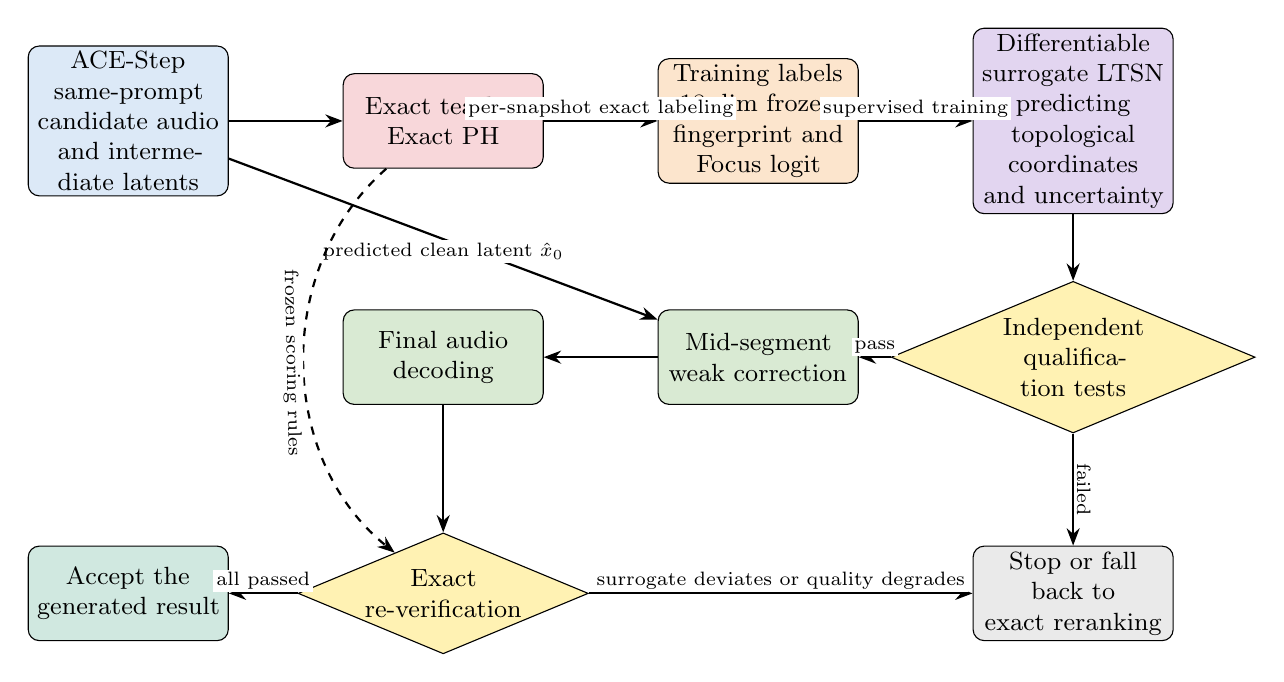
\begin{tikzpicture}[
    >={Stealth[length=2.2mm]},
    box/.style={draw, rounded corners, align=center,
                minimum height=12mm, text width=24mm,
                font=\small, fill=white, inner sep=2pt},
    decision/.style={draw, diamond, align=center, aspect=2.4,
                     text width=20mm, font=\small, fill=white, inner sep=1pt},
    arr/.style={->, thick},
    darr/.style={->, thick, dashed},
    lbl/.style={font=\scriptsize, fill=white, inner sep=1pt},
]
% ---- Node background colors grouped by role ----
% Input/data: light blue; exact teacher: light red; label artifacts: light orange;
% surrogate model: light purple; decision checks: light yellow; correction/decoding: light green;
% terminal acceptance: light cyan; fallback tier: light gray
\definecolor{cin}{HTML}{DCE9F7}      % input/candidates
\definecolor{cteacher}{HTML}{F8D7DA}  % exact teacher
\definecolor{clabel}{HTML}{FCE5CD}    % training labels
\definecolor{cproxy}{HTML}{E2D5F0}    % differentiable surrogate
\definecolor{cdecision}{HTML}{FFF2B3} % decision checks
\definecolor{cact}{HTML}{D9EAD3}     % correction/decoding actions
\definecolor{caccept}{HTML}{D0E8E0}  % accepted result
\definecolor{cback}{HTML}{EAEAEA}     % fallback tier
% ---- Main pipeline (top row L->R, bottom row R->L) ----
\node[box, fill=cin]        (A) at (0, 0)   {ACE-Step same-prompt\\candidate audio and intermediate latents};
\node[box, fill=cteacher]   (B) at (4, 0)   {Exact teacher\\Exact PH};
\node[box, fill=clabel]     (C) at (8, 0)   {Training labels\\18-dim frozen fingerprint and Focus logit};
\node[box, fill=cproxy]     (E) at (12, 0)  {Differentiable surrogate LTSN\\predicting topological coordinates and uncertainty};
\node[decision, fill=cdecision] (F) at (12, -3) {Independent qualification tests};
\node[box, fill=cact]       (G) at (8, -3)  {Mid-segment weak correction};
\node[box, fill=cact]       (H) at (4, -3)  {Final audio decoding};
\node[decision, fill=cdecision] (I) at (4, -6)  {Exact re-verification};
\node[box, fill=caccept]    (J) at (0, -6)  {Accept the generated result};
% ---- Upper branch: candidate reranking and fallback tier ----
% \node[box] (D) at (3.4, 3.4)    {Candidate reranking\\Exact best-of-$N$};
\node[box, fill=cback]      (K) at (12, -6) {Stop or fall back to\\exact reranking};

% ---- Solid arrows ----
\draw[arr] (A) -- (B);
\draw[arr] (B) -- node[lbl, above]{per-snapshot exact labeling} (C);
% \draw[arr] (B) -- node[lbl, right]{same-prompt exact scoring} (D);
\draw[arr] (C) -- node[lbl, above]{supervised training} (E);
\draw[arr] (E) -- (F);
\draw[arr] (F) -- node[lbl, above]{pass} (G);
\draw[arr] (G) -- (H);
\draw[arr] (H) -- (I);
\draw[arr] (I) -- node[lbl, above]{all passed} (J);
\draw[arr] (F) -- node[lbl, sloped, above]{failed} (K);
\draw[arr] (I) -- node[lbl, sloped, above, align=center]{surrogate deviates or quality degrades} (K);
\draw[arr] (A) to
    node[lbl, below, align=center]{predicted clean latent $\hat{x}_0$} (G);

% ---- Dashed arrows: frozen rules and fallback ----
\draw[darr] (B) to[bend right=50]
    node[lbl, sloped, below]{frozen scoring rules} (I);
% \draw[darr] (K) -- node[lbl, above]{retain the reliable tier} (D);
\end{tikzpicture}%
}
\caption{The exact teacher, differentiable surrogate, exact re-verification closed loop.}
\label{fig:acestep_pipeline}
\end{figure}

The generation side proceeds in the following gated order: first, the $18$-dimensional exact scorer is rebuilt and frozen; trajectories are then saved in a shadow mode that does not alter the generation results; next, it is checked whether the same-prompt candidate pool contains differences that the exact scorer can stably identify; only when exact reranking is effective are the LTSN trained and tested; finally, a weak-gradient corrector is developed. This order places ``whether the candidate space is identifiable'' and ``whether the surrogate can faithfully approximate it'' before sampling control, avoiding the use of complex guidance to mask a target that is itself unidentifiable.

\subsection{Frozen Objective and Target-Band Loss}

Let the generated audio be $x$; its frozen fingerprint is
\begin{equation}
z(x)=\Phi_{\mathrm{PH}}(x)
=\frac{1}{\sqrt{2}}\left[L(x)\Vert P(x)\right]\in\mathbb{R}^{18},
\end{equation}
where $L=Z_{\mathrm{Pitch}}\in\mathbb{R}^{16}$ and
$P=\frac{1}{\sqrt{2}}[Z_{\mathrm{Acoustic}}\Vert
Z_{\mathrm{Chroma}}]\in\mathbb{R}^{2}$.

On the discovery/180s data, the frozen L2 logistic regression reads the fingerprint out as a Focus decision logit:
\begin{equation}
S_F(x)=w^{\top}z(x)+b,\qquad p_F(x)=\sigma(S_F(x)).
\end{equation}
To prevent the guidance from raising the logit without bound, this paper determines the lower bound $\tau_F$ of the target band from a prespecified low quantile of the discovery Focus logits, and defines
\begin{equation}
L_{\mathrm{PH}}(x)=\left[\max\left(0,\tau_F-S_F(x)\right)\right]^2.
\label{eq:focus_band_loss}
\end{equation}
Once a sample enters the target band, the gradient becomes zero. Therefore, the control objective is to enter the neighborhood of the empirically supported Focus distribution, not to push any topological coordinate to an extreme.

\subsection{Inputs and Time Conditioning}

The acoustic latent variables of ACE-Step 1.5 XL-Turbo are $64$-dimensional, denoted $x_t\in\mathbb{R}^{B\times T\times64}$. A 180s audio corresponds to $T= 180 \times 25 = 4500$ at a latent time resolution of about 25Hz. The input of the LTSN is the $\hat{x}_0$ of each sampling step itself, rather than only the final \texttt{pred\_latents}. The input must be constructed from the real $x_t$, velocity $v_t$, and noise time $t$ to form $\hat x_0$. For a flow matching model, the corresponding predicted clean latent variable is
\begin{equation}
\hat{x}_0=x_t-tv_t.
\label{eq:pred_clean_latent}
\end{equation}

\begin{figure}[htbp]
    \centering
    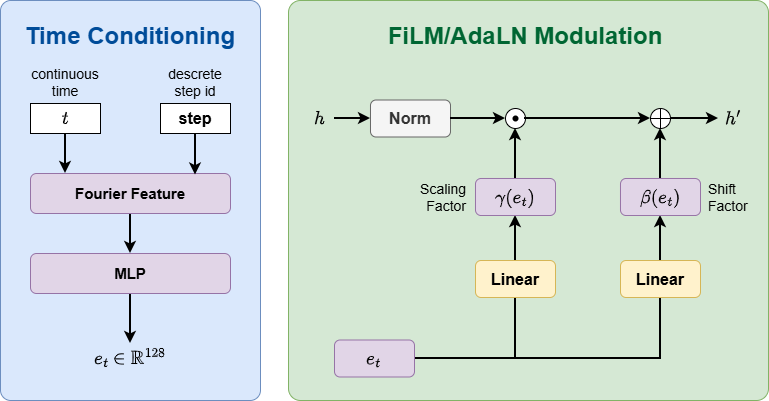
\includegraphics[width=0.8\textwidth]{fig/time_conditioning.png}
    \caption{Time conditioning module of the LTSN.}
    \label{fig:time_conditioning}
\end{figure}

A latent error of the same magnitude has different meanings at different noise times. The continuous time $t$ and the discrete step id are therefore encoded by Fourier features and a two-layer MLP into a $128$-dimensional conditioning vector:
\begin{equation}
e_t=\operatorname{MLP}(\operatorname{Fourier}(t,\text{step}))
\in\mathbb R^{128},
\end{equation}
which modulates the temporal residual blocks through FiLM/AdaLN:
\begin{equation}
\operatorname{FiLM}(h,e_t)=\gamma(e_t)\odot\operatorname{Norm}(h)+\beta(e_t).
\end{equation}

\subsection{The Latent Topology Surrogate Network (LTSN)}

\begin{figure}[htbp]
    \centering
    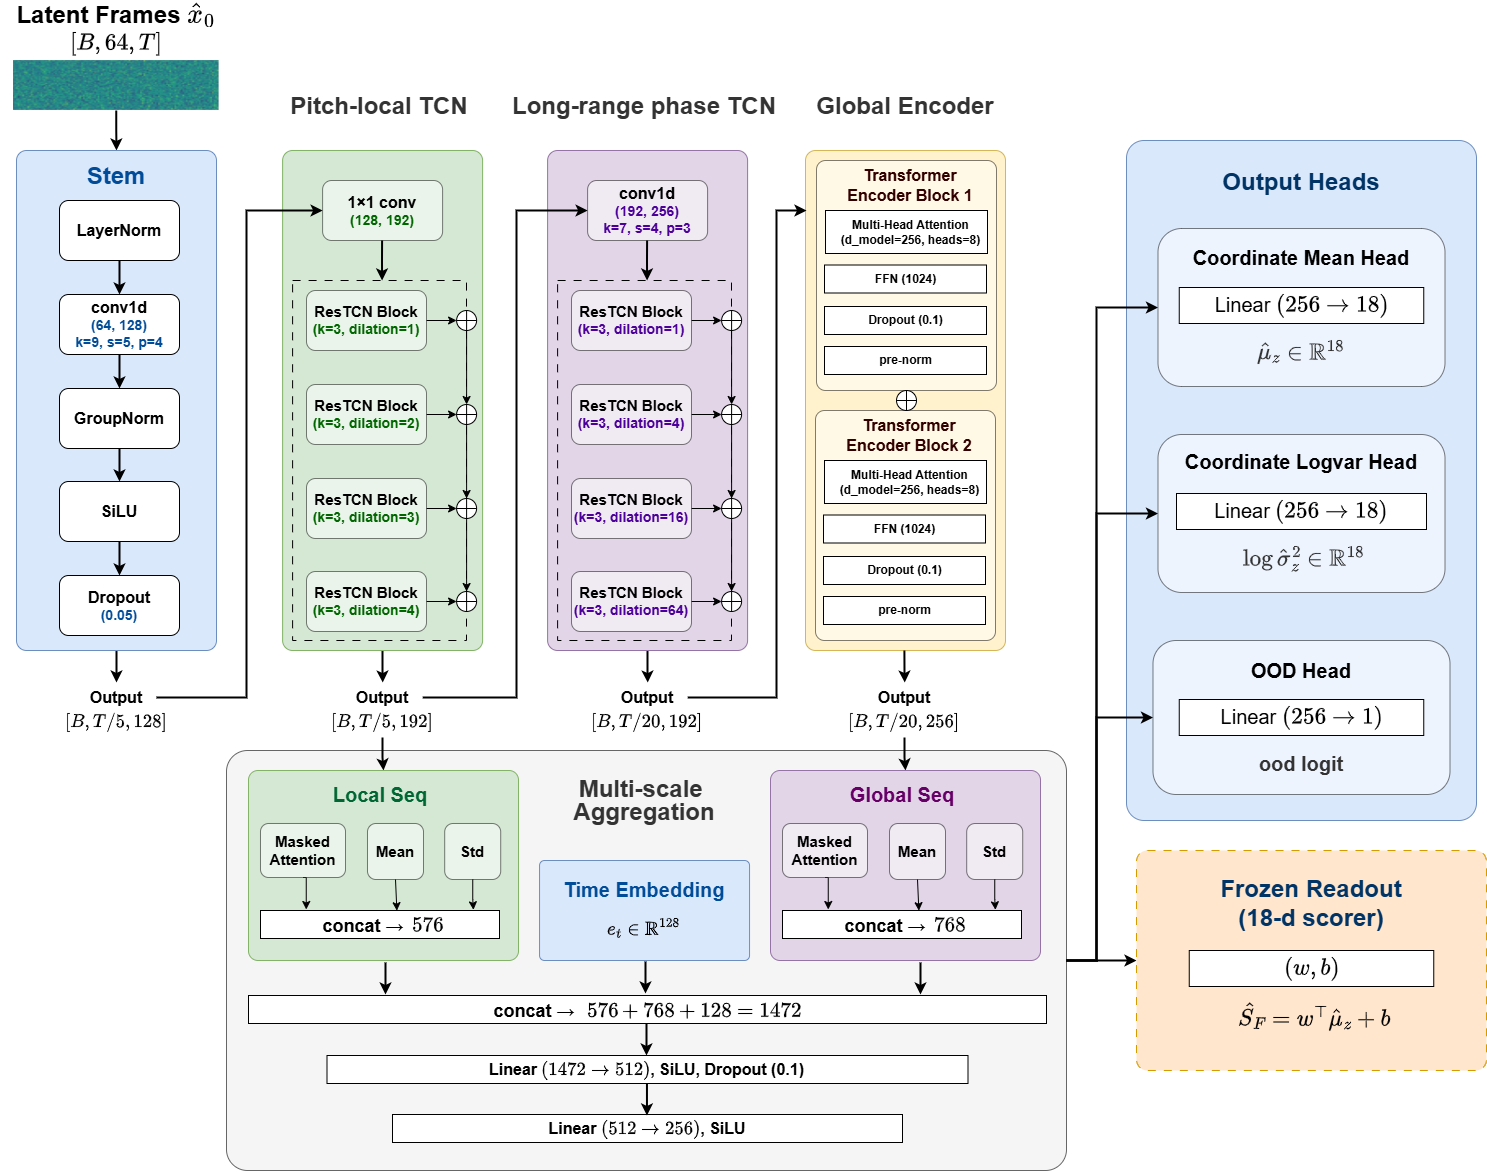
\includegraphics[width=\textwidth]{fig/architecture.png}
    \caption{Architecture of the LTSN.}
    \label{fig:ltsn_architecture}
\end{figure}

% \begin{table}[htbp]
% \centering
% \caption{LTSN network structure. $T$ is the number of input latent frames.}
% \label{tab:ltsn_architecture}
% \setlength{\tabcolsep}{4pt}
% \begin{tabular}{p{0.19\linewidth}p{0.42\linewidth}p{0.29\linewidth}}
% \toprule
% Module & Configuration & Output and function \\
% \midrule
% Stem & LayerNorm; Conv1d$(64,128,k=9,s=5)$; GroupNorm, SiLU, dropout $0.05$ &
% $[B,T/5,128]$; integrates local latent frames of about $0.36$s \\
% Pitch-local TCN & $1\times1$ projection to $192$ channels; four depthwise-separable residual blocks,
% $k=3$, dilation $=1,2,4,8$ & $[B,T/5,192]$; models local Pitch state transitions \\
% Long-range phase TCN & Conv1d$(192,256,k=7,s=4)$; four residual blocks, dilation
% $=1,4,16,64$ & $[B,T/20,256]$; covers recurrence over seconds to tens of seconds \\
% Global encoder & two-layer pre-norm Transformer, $d=256$, $8$ heads, FFN $=1024$ &
% connects distant Acoustic/Chroma phase positions \\
% Multi-scale pooling & masked attention, mean, and standard deviation pooling
% on the local and global sequences separately & $576+768$ dims \\
% Fusion layer & concatenates the $128$-dim time embedding; MLP $1472\rightarrow512\rightarrow256$ &
% $256$-dim shared representation \\
% Output heads & coordinate mean $18$ dims, log-variance $18$ dims, OOD logit $1$ dim &
% the Focus logit is computed by the frozen linear readout \\
% \bottomrule
% \end{tabular}
% \end{table}

\subsubsection{Stem}

The structure of the Stem can be summarized as:
\[\hat{x}_0 \to \texttt{LayerNorm} \to \texttt{Conv1d} \to \texttt{GroupNorm} \to \texttt{SiLU} \to \texttt{Dropout(0.05)}\]
It mainly accomplishes two tasks:
\begin{itemize}
    \item expanding the $64$-dimensional acoustic latent variables to $128$-dimensional features;
    \item downsampling the 25 Hz latent variables to 5 Hz.
\end{itemize}
The \verb|Conv1d| parameters are \verb|(64, 128, kernel=9, stride=5, padding=4)|. With \verb|kernel = 9|, at 25 Hz this corresponds to $9/25=0.36 \text{s}=360 \text{ms}$, and \verb|stride = 5| corresponds to $5/25=0.2s=200ms$. Each output frame therefore covers about $360$ ms of input context, and consecutive output frames are $200$ ms apart. The final output features are $[B, T/5, 128]$.

\subsubsection{Pitch-Local TCN}

After the Stem, a $1 \times 1$ convolution projects the features to $192$ channels, followed by four residual TCN blocks in series:

\begin{table}[htbp]
\centering
\caption{Configuration of the Pitch-local TCN residual blocks}
\renewcommand{\arraystretch}{1.5}
\setlength{\tabcolsep}{8pt}
\begin{tabular}{lrrrr}
\toprule
block & \texttt{kernel} & \texttt{dilation} & Channels & Function  \\
\midrule
\#1     & $3$      & $1$        & $192$  & Local adjacent tokens    \\
\#2     & $3$      & $2$        & $192$  & Short-term harmonic state changes  \\
\#3     & $3$      & $4$        & $192$  & Local organization over seconds     \\
\#4     & $3$      & $8$        & $192$  & Longer local context   \\
\bottomrule
\end{tabular}
\end{table}

The internal structure of each block is:
\begin{figure}[htbp]
    \centering
    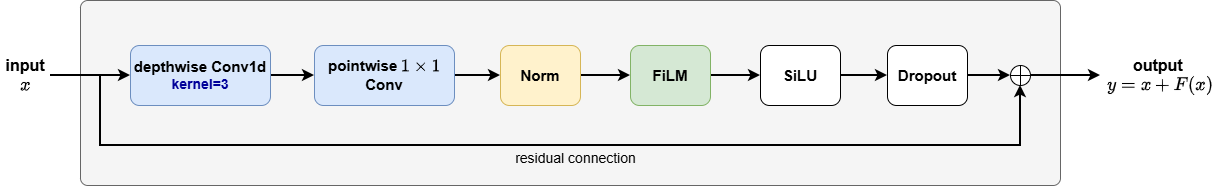
\includegraphics[width=\textwidth]{fig/tcn_block.png}
    \caption{Architecture of a TCN residual block.}
    \label{fig:tcn_block}
\end{figure}

As the \verb|dilation| increases, the receptive field keeps growing. With the four blocks in series, the deepest view covers about $3.4$ seconds of context, corresponding to ``local organization over seconds'' and ``local context''.

\subsubsection{Long-Range Phase TCN}

The Long-range phase TCN follows the Pitch-local TCN and captures repeating structures and phase relations over longer time scales. The local features are first downsampled to $1.25$ Hz by \texttt{Conv1d(192,256,kernel=7,stride=4)}, with a time interval of about $4 \times 0.2 = 0.8s$; four $256$-channel residual TCN blocks with the same structure as those of the Pitch-local TCN are then connected in series, with \texttt{dilation} $1, 4, 16, 64$, respectively. After the four residual blocks, the receptive field can cover repeating structures and phase relations from a few seconds to over a hundred seconds. The final output features of the Long-range phase TCN are $[B, T/20, 256]$.

\subsubsection{Global Encoder}

After the Stem downsamples the sequence to $900$ tokens and the Long-range phase TCN further downsamples it to about $225$ tokens, a Transformer can perform full-length self-attention at low cost to capture repetition relations that are far apart. Here we use two pre-norm Transformer encoder blocks:
\[\underbrace{\texttt{d\_model=256, heads=8, FFN=1024, dropout=0.1, pre-norm}}_{\times 2}\]
Each block does not change the sequence length or the feature dimension, so the output shape remains $[B, T/20, 256]$.

\subsubsection{Multi-Scale Pooling and Shared Representation}

The preceding network produces two sequences at different scales:
\begin{itemize}
    \item \textbf{Local sequence}: high time resolution, good at capturing details within a few seconds; output shape $[B, T/5, 192]$;
    \item \textbf{Global sequence}: low time resolution, good at capturing structures over tens of seconds or even the whole track; output shape $[B, T/20, 256]$.
\end{itemize}
This module pools the two sequences into compact vectors separately, concatenates them with the time embedding $e_t \in \mathbb{R}^{128}$, and passes the result through a small MLP to obtain a shared representation for the subsequent tasks.

For either the local or the global sequence $h$, the multi-scale pooling is written as
\begin{equation}
p(h)=\left[p_{\mathrm{attn}}(h)\Vert\operatorname{mean}(h)
\Vert\operatorname{std}(h)\right].
\end{equation}
The local pooling has $192\times3=576$ dimensions and the global pooling has $256\times3=768$ dimensions; concatenated with $e_t$, they give a fused input of $576+768+128=1472$ dimensions. The concatenated $1472$-dimensional vector passes through two linear layers:
\[\texttt{Linear(1472,512)} \to \texttt{SiLU} \to \texttt{Dropout(0.1)} \to \texttt{Linear(512,256)} \to \texttt{SiLU}\]
finally yielding a $256$-dimensional shared representation.

\subsubsection{Output Heads and Frozen Readout}

The LTSN learns a heteroscedastic conditional distribution
\begin{equation}
g_{\phi}(\hat{x}_0,t)\longrightarrow
(\hat{\mu}_z,\log\hat{\sigma}_z^2,u_{\mathrm{OOD}}),
\end{equation}
where:
\begin{table}[htbp]
\centering
\caption{Output heads}
\renewcommand{\arraystretch}{1.5}
\begin{tabular}{lccp{8cm}}
\toprule
name & Symbol & Dim & Function  \\
\midrule
\texttt{coordinate\_mean\_head}     & $\hat{\mu}_z$      & $18$    & predicts the mean of each latent coordinate $z$   \\
\texttt{coordinate\_logvar\_head}   & $\log\hat{\sigma}_z^2$      & $18$    & predicts the log-variance of each coordinate dimension, expressing the model's uncertainty about its own predictions   \\
\texttt{ood\_head}     & $u_{\mathrm{OOD}}$      & $1$        & expresses the probability that the input sample is out of distribution     \\
\bottomrule
\end{tabular}
\end{table}

The Focus logit does not have an independent classification head that could freely deviate from the coordinates; it is computed deterministically from the frozen parameters:
\begin{equation}
\hat{S}_F=w^{\top}\hat{\mu}_z+b.
\label{eq:ltsn_frozen_readout}
\end{equation}
This design keeps the surrogate coordinates consistent with the overall score, preventing the network from catering only to the overall logit while corrupting the Pitch or the two phase coordinates.

This paper trains three members with identical architectures and data but different random seeds; the single-model variance characterizes the aleatoric uncertainty, and the cross-member variance characterizes the epistemic uncertainty.

\subsection{Teacher Labels, Data Construction, and Leakage-Proof Splitting}

One training sample of the LTSN consists of $(\hat{x}_0,t,z,S_F,y_{\mathrm{OOD}})$. Label generation must be performed independently for each trajectory snapshot: during unguided generation, the $(x_t,v_t,t)$ of steps 4, 5, 6 and the final step are saved; the corresponding $\hat{x}_0$ values are constructed according to Equation~\eqref{eq:pred_clean_latent}; each is decoded by the VAE separately; the exact Pitch PH, Acoustic phase, and Chroma phase pipelines are then run independently, and finally the frozen transformations produce the snapshot's own $z$ and $S_F$.
% The label of the final audio must not be copied to all intermediate steps, otherwise the network would learn an incorrect time-invariant mapping.

The data consist of three parts:
\begin{enumerate}
    \item VAE reconstructions of the $195$ Focus and $195$ Classical tracks in the discovery set, serving as real-music anchors;
    \item unguided 180s trajectories of no fewer than $512$ development prompts with $4$ seeds per prompt, each trajectory labeled at steps 4, 5, 6 and the final step, forming about $8192$ generated snapshots;
    \item safety/OOD negative examples accounting for $10\%$--$15\%$ of the training batches, including silence, clipping, extremely low dynamics, mechanical short loops, over-smoothing, and abnormal latents.
\end{enumerate}

To avoid trajectory leakage, the real audio is grouped by track and the generated samples are grouped by prompt; all seeds and snapshots of the same track, the same prompt, or the same generation trajectory must lie in the same partition. The training, development, and calibration partitions account for $70\%$, $15\%$, and $15\%$ of the prompt groups, respectively; in addition, qualification prompts are set aside that do not participate in parameter fitting, architecture selection, early stopping, or threshold calibration. The paper's validation and the already opened holdout are used only for the frozen topological evidence, and are not used for architecture selection, loss reweighting, or qualification-threshold adjustment of the LTSN.

\subsection{Loss Functions and Training}

Directly averaging the $18$ coordinates would let the $16$-dimensional Pitch block dominate the optimization because of its higher dimensionality. This paper defines a block-balanced coordinate loss according to the frozen distance weights:
\begin{equation}
L_{\mathrm{coord}}={}
\frac{1}{2} \times \frac{1}{16}\sum_{j\in L}
\operatorname{Huber}(\hat{\mu}_j-z_j)
+\frac{1}{4}\operatorname{Huber}(\hat{\mu}_A-z_A)
+\frac{1}{4}\operatorname{Huber}(\hat{\mu}_C-z_C).
\label{eq:block_balanced_loss}
\end{equation}
Let $s_j=\log\hat{\sigma}_j^2$; the heteroscedastic negative log-likelihood is
\begin{equation}
L_{\mathrm{NLL}}=
\sum_{b\in\{L,A,C\}}\omega_b\frac{1}{d_b}\sum_{j\in b}
\frac{1}{2}\left[e^{-s_j}(z_j-\hat{\mu}_j)^2+s_j\right],
\end{equation}
where $(\omega_L,\omega_A,\omega_C)=(1/2,1/4,1/4)$, and $s_j$ is constrained to a prespecified interval so that the network cannot evade errors by inflating the variance without bound. The consistency loss of the frozen readout is
\begin{equation}
L_{\mathrm{score}}=\operatorname{Huber}(\hat{S}_F-S_F).
\end{equation}
For same-prompt candidates $(i,k)$ whose exact score difference exceeds a prespecified margin, a logistic ranking loss is used:
\begin{equation}
L_{\mathrm{rank}}=\log\left(1+
\exp\left[-y_{ik}(\hat{S}_i-\hat{S}_k)/\tau_r\right]\right),
\quad y_{ik}=\operatorname{sign}(S_i-S_k).
\end{equation}
Adjacent snapshots are not artificially required to be smooth; instead, they are matched to the exact trajectory increments:
\begin{equation}
L_{\Delta}=\operatorname{Huber}\left[
(\hat{\mu}_{s+1}-\hat{\mu}_s)-(z_{s+1}-z_s)\right].
\end{equation}
The safety negative examples use binary cross-entropy $L_{\mathrm{OOD}}$. The prespecified total loss at the development stage is
\begin{equation}
L=L_{\mathrm{coord}}+0.25L_{\mathrm{NLL}}+0.5L_{\mathrm{score}}
+0.2L_{\mathrm{rank}}+0.2L_{\Delta}+0.1L_{\mathrm{OOD}}.
\label{eq:ltsn_total_loss}
\end{equation}
% The coefficients in Equation~\eqref{eq:ltsn_total_loss} are a development starting point rather than a validated conclusion; they may be selected only once on the independent development prompts and are frozen together with the network architecture, the data inventory, and
% all hashes before qualification.

Training uses AdamW with an initial learning rate of $3\times10^{-4}$ and a weight decay of $10^{-2}$, with cosine decay to $10^{-6}$ after $5\%$ warmup; forward and backward propagation are executed in bf16, while losses and variance computations remain in fp32; the batch size per GPU is $8$--$16$, with gradient accumulation to an effective batch of $64$ and global gradient-norm clipping at $1.0$. The sampler is balanced over steps 4, 5, 6 and the final step, Focus logit quantiles, and the OOD proportion. Early stopping considers both the development score error and the block-level Spearman correlations of Pitch/Phase. During training, only the precomputed latents and exact labels are read, and neither the ACE-Step DiT nor the VAE is loaded; the 180s latents are not randomly cropped while keeping the whole-track labels, and shuffling the temporal order is not used as data augmentation.

\begin{tcolorbox}[colback=yellow!30,colframe=yellow!60,boxrule=0.5pt,arc=6pt,left=6pt,right=6pt,top=4pt,bottom=4pt]
TODO: The surrogate model training is not yet complete; it is planned to be trained on L40s GPUs.
\end{tcolorbox}

\subsection{Sampling-Time Topological Correction}

ACE-Step Turbo is a CFG-distilled model, so \texttt{guidance\_scale} is not the topological control interface of this paper. During sampling, the DiT always remains in \texttt{no\_grad}; only the predicted clean latent variable obtained from Equation~\eqref{eq:pred_clean_latent} is detached from the main graph and given gradients:
\begin{equation}
\tilde{x}_0=\operatorname{stopgrad}(x_t-tv_t),\qquad
\tilde{x}_0.\mathrm{requires\_grad}=\mathrm{True}.
\end{equation}
The surrogate energy is written as
\begin{equation}
\mathcal{E}_t=
\left[\max(0,\tau_F-\hat{S}_F(\tilde{x}_0,t))\right]^2
+\lambda_uU_{\mathrm{OOD}}+\lambda_qL_{\mathrm{quality}}.
\end{equation}
The uncertainty and quality terms are used only to trigger no-op or impose safety constraints, and do not change the composition of the frozen topological objective. For a valid-frame mask $M$, the correction direction is
\begin{equation}
g_t=\nabla_{\tilde{x}_0}\mathcal{E}_t,\qquad
\delta_t=-\eta_k\operatorname{LPF}(M\odot g_t),
\end{equation}
where the LPF suppresses frame-by-frame high-frequency perturbations. A relative RMS clipping is then applied to each sample:
\begin{equation}
\delta_t\leftarrow\delta_t\min\left(1,
\frac{\rho\operatorname{RMS}(\tilde{x}_0)}
{\operatorname{RMS}(\delta_t)+\epsilon}\right),
\end{equation}
and the result is mapped to the next noise time:
\begin{equation}
x_{t_{\mathrm{next}}}\leftarrow x_{t_{\mathrm{next}}}
+(1-t_{\mathrm{next}})a_k\delta_t.
\label{eq:topology_corrector_update}
\end{equation}

The default 8-step time sequence with shift$=3.0$ is
$[1.000,0.955,0.900,0.833,0.750,0.643,0.500,0.300]$. The initial design enables correction only at steps 4--6, with inter-step weights $a_k=[0.5,1.0,0.5]$, thereby avoiding the first three high-noise steps and the last step that directly outputs $x_0$. The RMS upper bound is selected only once on the independent development prompts from the three prespecified values $0.25\%$, $0.5\%$, and $1.0\%$ of the latent RMS.

In the sampling loop, the corrector is placed after the Euler/Heun base update and DCW and before the Repaint injection; Repaint always runs last so that the protected regions are not overwritten by the topological gradient. The correction must degrade to an identity mapping on a per-sample basis whenever the scorer or model hashes do not match, the step is outside the window, the strength is zero, the ensemble disagreement or prediction interval exceeds the threshold, the sample is OOD, NaN/Inf occurs, or the padding/Repaint mask is invalid.

\subsection{Qualification Tests and Final Evaluation}

The LTSN is allowed into the sampler only if it simultaneously satisfies the following thresholds on unseen prompts, seed families, and trajectories: a Focus logit Spearman $\rho\geq0.70$; a median Spearman $\rho\geq0.50$ across the $18$ coordinates; correlations of both the Pitch block distance and the Phase block distance no lower than $0.50$; correlations of both the Acoustic and Chroma \texttt{loop\_score} values no lower than $0.50$; a ranking accuracy on the exact top/bottom quartiles no lower than $0.65$; a $90\%$ prediction-interval coverage within $0.85$--$0.95$; reliable no-op triggering on OOD or high-uncertainty samples; and, after surrogate-gradient optimization, the exact score and the surrogate score of the decoded audio improving in the same direction. Failure of any single main block cannot be masked by the overall logit correlation.

The final confirmation uses $32$ new prompts with $8$ seeds per prompt, and generates a baseline/guided pair for each seed, totaling $512$ 180s audio clips. The primary endpoint is
\begin{equation}
\Delta_i=L_{\mathrm{PH}}^{\mathrm{guided}}(i)
-L_{\mathrm{PH}}^{\mathrm{base}}(i),
\end{equation}
where negative values indicate closer proximity to the frozen target band. The report includes the median difference, the Hodges--Lehmann shift, the prompt-clustered bootstrap $95\%$ confidence interval, and the target-band hit rate; at the same time, prespecified non-inferiority tests are performed on prompt consistency, LUFS, true peak, clipping, silence, spectral anomalies, mechanical short loops, over-smoothing, diversity, blind-listening audio quality, runtime, and memory. Even if exact PH improves, the guidance is still judged a failure as long as audio quality, prompt consistency, or diversity crosses the boundary.

\begin{tcolorbox}[colback=yellow!30,colframe=yellow!60,boxrule=0.5pt,arc=6pt,left=6pt,right=6pt,top=4pt,bottom=4pt]
TODO: The final evaluation can only start after the LTSN training is complete. The methods and criteria are recorded here first, and the report will be supplemented after the tests are finished.
\end{tcolorbox}

\begin{tcolorbox}[colback=yellow!30,colframe=yellow!60,boxrule=0.5pt,arc=6pt,left=6pt,right=6pt,top=4pt,bottom=4pt]
QUESTION: Is a human listening experiment needed? There may not be enough time, and it may involve ethics approval.
\end{tcolorbox}

\clearpage

\bibliography{biblio.bib}


%%%%%%%%%%%%%%%%%%%%%%%%%%%%%%%%%%%%%%%%%%%%%%%%%%%%%%%%%%%%
\clearpage
\appendix

\section{Complete Feature Metric Data}
\label{sec:appendix_topology_tables}

This appendix provides the complete topological feature comparison data of classical music and focus music under the pitch, rhythm, and modulation views. The metrics are sorted in descending order of $\epsilon^2$ from the 180s primary analysis; $\epsilon^2$ is the Kruskal--Wallis rank effect size, and the BH-FDR $q$ is the Benjamini-Hochberg adjusted $p$-value of the raw $p$-value within the prespecified test family. The independent pairwise comparisons additionally report the rank-biserial effect size.

\subsection{Pitch View}

\begin{table}[htbp]
\centering
\caption{Topological feature comparison of classical music and focus music in the pitch view}
\label{tab:pitch_topology}
\renewcommand{\arraystretch}{1.5}
\begin{tabular}{lrrrrr}
\toprule
Metric                    & $\text{Median}_{\text{Classical}}$ & $\text{Median}_{\text{Focus}}$ & $\epsilon^2$ & 180s BH-FDR $q$ & 300s BH-FDR $q$ \\
\midrule
\rowcolor{green!15}\verb|vertex_count|            &           16.000 &            10.000 &        0.703 &   8.2e-19 &   2.8e-19 \\
\rowcolor{green!15}\verb|edge_count|              &           70.000 &            31.000 &        0.683 &   8.2e-19 &   1.8e-19 \\
\rowcolor{green!15}\verb|h0_betti_auc|            &            6.200 &             3.125 &        0.677 &   8.2e-19 &   1.8e-19 \\
\rowcolor{green!15}\verb|h0_betti_mean|           &           13.667 &             6.833 &        0.676 &   8.2e-19 &   1.8e-19 \\
\rowcolor{green!15}\verb|h0_observed_persistence| &            6.375 &             3.325 &        0.677 &   8.2e-19 &   1.8e-19 \\
\rowcolor{green!15}\verb|h0_betti_max|            &           14.500 &             8.000 &        0.672 &   8.2e-19 &   1.8e-19 \\
\rowcolor{green!15}\verb|h0_interval_count|       &           14.500 &             8.000 &        0.672 &   8.2e-19 &   1.8e-19 \\
\rowcolor{green!15}\verb|path_entropy|            &            1.696 &             0.965 &        0.673 &   8.2e-19 &   1.8e-19 \\
\rowcolor{green!15}\verb|h0_censored_count|       &           11.000 &             3.500 &        0.596 &  6.53e-17 &  7.59e-18 \\
\rowcolor{green!15}\verb|directed_recurrence|     &            0.025 &             0.114 &        0.585 &  1.14e-16 &  4.43e-17 \\
\rowcolor{green!15}\verb|self_transition_ratio|   &            0.322 &             0.631 &        0.563 &  3.89e-16 &  1.92e-16 \\
\rowcolor{green!15}\verb|transition_entropy|      &            0.915 &             0.771 &        0.489 &  3.03e-14 &  8.01e-14 \\
\rowcolor{green!15}\verb|reciprocity|             &            0.522 &             0.667 &        0.361 &  6.25e-11 &  2.31e-09 \\
\verb|edge_density|            &            0.311 &             0.332 &        0.025 &    0.0654 &         1 \\
\rowcolor{orange!15}\verb|h1_betti_auc|            &            0.000 &             0.000 &        0.010 &     0.153 &    0.0255 \\
\rowcolor{orange!15}\verb|h1_betti_max|            &            0.000 &             0.000 &        0.010 &     0.153 &    0.0255 \\
\rowcolor{orange!15}\verb|h1_betti_mean|           &            0.000 &             0.000 &        0.010 &     0.153 &    0.0255 \\
\rowcolor{orange!15}\verb|h1_censored_count|       &            0.000 &             0.000 &        0.010 &     0.153 &    0.0255 \\
\rowcolor{orange!15}\verb|h1_interval_count|       &            0.000 &             0.000 &        0.010 &     0.153 &    0.0255 \\
\verb|h1_observed_persistence| &            0.000 &             0.000 &        0.000 &         1 &         1 \\
\bottomrule
\end{tabular}
\end{table}

% \vspace{2em}

\begin{table}[htbp]
\centering
\caption{Metrics of the pitch view that pass the independent pairwise FDR (Open Focus-Classical, 180s)}
\label{tab:pitch_rank_biserial}
\renewcommand{\arraystretch}{1.5}
\makebox[\linewidth][c]{%
  \begin{tabular}{lrr||lrr}
    \toprule
    Metric & rank-biserial & BH-FDR $q$ & Metric & rank-biserial & BH-FDR $q$ \\
    \midrule
    \texttt{edge\_count} & -0.956 & 8.4e-19 & \texttt{vertex\_count} & -0.954 & 8.4e-19 \\
    \texttt{h0\_betti\_auc} & -0.952 & 8.4e-19 & \texttt{h0\_censored\_count} & -0.892 & 6.68e-17 \\
    \texttt{h0\_betti\_max} & -0.944 & 8.4e-19 & \texttt{directed\_recurrence} & 0.886 & 1.16e-16 \\
    \texttt{h0\_betti\_mean} & -0.951 & 8.4e-19 & \texttt{self\_transition\_ratio} & 0.869 & 3.97e-16 \\
    \texttt{h0\_interval\_count} & -0.944 & 8.4e-19 & \texttt{transition\_entropy} & -0.811 & 3.09e-14 \\
    \texttt{h0\_observed\_persistence} & -0.952 & 8.4e-19 & \texttt{reciprocity} & 0.699 & 6.37e-11  \\
    \texttt{path\_entropy} & -0.949 & 8.4e-19 &  &  &  \\
    \bottomrule
  \end{tabular}%
}
\end{table}

\clearpage
\subsection{Rhythm View}

\begin{table}[htbp]
\centering
\caption{Topological feature comparison of classical music and focus music in the rhythm view}
\label{tab:rhythm_topology}
\renewcommand{\arraystretch}{1.5}
\begin{tabular}{lrrrrr}
\toprule
Metric                    & $\text{Median}_{\text{Classical}}$ & $\text{Median}_{\text{Focus}}$ & $\epsilon^2$ & 180s BH-FDR $q$ & 300s BH-FDR $q$ \\
\midrule
\rowcolor{green!15}\verb|path_entropy|            &            1.336 &             0.866 &        0.390 &  1.38e-10 &  1.06e-10 \\
\rowcolor{green!15}\verb|edge_count|              &           36.000 &            21.000 &        0.356 &  5.48e-10 &  3.06e-10 \\
\rowcolor{green!15}\verb|directed_recurrence|     &            0.092 &             0.265 &        0.311 &  5.47e-09 &  1.78e-08 \\
\rowcolor{green!15}\verb|h0_betti_mean|           &            6.833 &             4.750 &        0.299 &  8.56e-09 &  4.62e-09 \\
\rowcolor{green!15}\verb|h0_betti_auc|            &            3.100 &             2.175 &        0.288 &  1.35e-08 &  4.62e-09 \\
\rowcolor{green!15}\verb|h0_observed_persistence| &            3.300 &             2.275 &        0.276 &  2.02e-08 &  4.62e-09 \\
\rowcolor{green!15}\verb|transition_entropy|      &            0.792 &             0.611 &        0.276 &  2.02e-08 &  4.82e-07 \\
\rowcolor{green!15}\verb|h0_betti_max|            &            8.000 &             6.000 &        0.256 &  5.13e-08 &  2.50e-08 \\
\rowcolor{green!15}\verb|h0_interval_count|       &            8.000 &             6.000 &        0.256 &  5.13e-08 &  2.50e-08 \\
\rowcolor{green!15}\verb|self_transition_ratio|   &            0.479 &             0.662 &        0.252 &  5.78e-08 &  3.15e-08 \\
\rowcolor{green!15}\verb|h0_censored_count|       &            5.000 &             2.000 &        0.245 &  8.46e-08 &  1.24e-05 \\
\rowcolor{green!15}\verb|vertex_count|            &            8.000 &             7.000 &        0.166 &  9.64e-06 &  1.83e-05 \\
\rowcolor{green!15}\verb|edge_density|            &            0.577 &             0.493 &        0.075 &    0.00267 &  1.84e-05 \\
\rowcolor{green!15}\verb|reciprocity|             &            0.809 &             0.769 &        0.039 &    0.0248 &    0.00639 \\
\verb|h1_observed_persistence| &            0.000 &             0.000 &        0.000 &    0.423 &         1 \\
\verb|h1_betti_auc|            &            0.000 &             0.000 &        0.000 &         1 &    0.334 \\
\verb|h1_betti_max|            &            0.000 &             0.000 &        0.000 &         1 &    0.334 \\
\verb|h1_betti_mean|           &            0.000 &             0.000 &        0.000 &         1 &    0.334 \\
\verb|h1_censored_count|       &            0.000 &             0.000 &        0.000 &         1 &    0.334 \\
\verb|h1_interval_count|       &            0.000 &             0.000 &        0.000 &         1 &    0.334 \\
\bottomrule
\end{tabular}
\end{table}

\vspace{2em}

\begin{table}[htbp]
\centering
\caption{Metrics of the rhythm view that pass the independent pairwise FDR (Open Focus-Classical, 180s)}
\label{tab:rhythm_rank_biserial}
\renewcommand{\arraystretch}{1.5}
\makebox[\linewidth][c]{%
  \begin{tabular}{lrr||lrr}
    \toprule
    Metric & rank-biserial & BH-FDR $q$ & Metric & rank-biserial & BH-FDR $q$ \\
    \midrule
    \texttt{path\_entropy} & -0.726 & 1.4e-10 & \texttt{h0\_betti\_max} & -0.580 & 5.21e-08 \\
    \texttt{edge\_count} & -0.694 & 5.58e-10 & \texttt{h0\_interval\_count} & -0.580 & 5.21e-08 \\
    \texttt{directed\_recurrence} & 0.650 & 5.56e-09 & \texttt{self\_transition\_ratio} & 0.587 & 5.86e-08 \\
    \texttt{h0\_betti\_mean} & -0.637 & 8.7e-09 & \texttt{h0\_censored\_count} & -0.570 & 8.59e-08 \\
    \texttt{h0\_betti\_auc} & -0.626 & 1.37e-08 & \texttt{vertex\_count} & -0.467 & 9.76e-06 \\
    \texttt{h0\_observed\_persistence} & -0.613 & 2.05e-08 & \texttt{edge\_density} & -0.331 & 0.0027 \\
    \texttt{transition\_entropy} & -0.613 & 2.05e-08 & \texttt{reciprocity} & -0.252 & 0.025  \\
    \bottomrule
  \end{tabular}%
}
\end{table}

\clearpage
\subsection{Modulation View}

\begin{table}[htbp]
\centering
\caption{Topological feature comparison of classical music and focus music in the modulation view}
\label{tab:modulation_topology}
\renewcommand{\arraystretch}{1.5}
\begin{tabular}{lrrrrr}
\toprule
Metric                    & $\text{Median}_{\text{Classical}}$ & $\text{Median}_{\text{Focus}}$ & $\epsilon^2$ & 180s BH-FDR $q$ & 300s BH-FDR $q$ \\
\midrule
\rowcolor{green!15}\verb|edge_density|            &            0.667 &             0.524 &        0.105 &    0.00509 &    0.0423 \\
\rowcolor{orange!15}\verb|h0_censored_count|       &            1.000 &             1.000 &        0.087 &    0.00533 &     0.159 \\
\rowcolor{green!15}\verb|vertex_count|            &            5.000 &             6.000 &        0.092 &    0.00533 &    0.0396 \\
\rowcolor{green!15}\verb|reciprocity|             &            0.873 &             0.776 &        0.078 &     0.0071 &    0.0464 \\
\rowcolor{green!15}\verb|edge_count|              &           11.500 &            14.000 &        0.051 &    0.0328 &    0.0424 \\
\rowcolor{orange!15}\verb|h0_betti_max|            &            4.000 &             5.000 &        0.035 &    0.0633 &    0.0424 \\
\rowcolor{orange!15}\verb|h0_betti_mean|           &            2.917 &             3.583 &        0.034 &    0.0633 &    0.0424 \\
\rowcolor{orange!15}\verb|h0_interval_count|       &            4.000 &             5.000 &        0.035 &    0.0633 &    0.0424 \\
\verb|self_transition_ratio|   &            0.448 &             0.401 &        0.031 &    0.0699 &    0.0928 \\
\rowcolor{orange!15}\verb|h0_betti_auc|            &            1.300 &             1.625 &        0.028 &    0.0747 &    0.0424 \\
\rowcolor{orange!15}\verb|h0_observed_persistence| &            1.450 &             1.775 &        0.026 &    0.0809 &    0.0424 \\
\rowcolor{orange!15}\verb|directed_recurrence|     &            0.130 &             0.109 &        0.021 &      0.1 &    0.0424 \\
\rowcolor{orange!15}\verb|transition_entropy|      &            0.843 &             0.860 &        0.010 &     0.216 &    0.0424 \\
\verb|path_entropy|            &            1.087 &             1.119 &        0.000 &     0.643 &     0.962 \\
\verb|h1_betti_auc|            &            0.000 &             0.000 &        0.000 &     0.683 &         1 \\
\verb|h1_betti_max|            &            0.000 &             0.000 &        0.000 &     0.683 &         1 \\
\verb|h1_betti_mean|           &            0.000 &             0.000 &        0.000 &     0.683 &         1 \\
\verb|h1_censored_count|       &            0.000 &             0.000 &        0.000 &     0.683 &         1 \\
\verb|h1_interval_count|       &            0.000 &             0.000 &        0.000 &     0.683 &         1 \\
\verb|h1_observed_persistence| &            0.000 &             0.000 &        0.000 &     0.683 &     0.453 \\
\bottomrule
\end{tabular}
\end{table}

\vspace{2em}

\begin{table}[h]
\centering
\caption{Metrics of the modulation view that pass the independent pairwise FDR (Open Focus-Classical, 180s)}
\label{tab:modulation_rank_biserial}
\renewcommand{\arraystretch}{1.5}
\begin{tabular}{lrr}
\toprule
Metric & rank-biserial & BH-FDR $q$ \\
\midrule
\verb|edge_density| & -0.386 & 0.00514 \\
\verb|h0_censored_count| & 0.299 & 0.00539 \\
\verb|vertex_count| & 0.355 & 0.00539 \\
\verb|reciprocity| & -0.336 & 0.00716 \\
\verb|edge_count| & 0.279 & 0.0331 \\
\bottomrule
\end{tabular}
\end{table}

%%%%%%%%%%%%%%%%%%%%%%%%%%%%%%%%%%%%%%%%%%%%%%%%%%%%%%%%%%%%
\clearpage

\section{Acknowledgments}

This research was completed almost independently by myself, with the support of several experts and teachers along the way, to whom I would like to express my gratitude.

I thank Mr. Tian'ang Xiao for teaching me the architecture of ACE-Step and the principles of LoRA training, which enabled me to know how to intervene in the generation of ACE-Step within a short time. Mr. Xiao got master degree in statistics from the University of Glasgow and focuses on Diffusion model research. The LTSN in this paper was completed with his assistance and guidance. He taught me how to build neural networks with pytorch and provided two L40s GPUs for model training.

I thank Associate Professor Jingheng Cai of the School of Mathematics at Sun Yat-sen University for his guidance on statistical methods. Professor Cai taught me many statistical tools and methods never covered in AP Statistics, especially between-group multivariate statistical analyses such as the Mann--Whitney $U$ test and PERMANOVA, which made the conclusions of this paper more convincing.

I thank Mr. Xiao'an Yang for his guidance on the writing of this paper. As my school advisor, Mr. Yang pointed out many places in the paper that were verbose or not rigorous, and he supervised and encouraged me to keep pushing the research forward.

Finally, I specially thank Dr. Zhaojun Chen and Dr. Kevin JP Woods. Dr. Zhaojun Chen is my senior schoolmate. She is currently pursuing a PhD in mathematics at Caltech, focusing on algebraic topology. When she visited back to school this year, she gave a topology lecture which inspired my idea of studying musical structure with topology. Dr. Woods is the director of science at Brain.fm, focusing on auditory attention and neuromodulation. He generously licensed Brain.fm's focus music for this research, which became the starting point of this work.

\clearpage

\section{Research Journey}

This research originated from my personal curiosity about Focus Music. As a heavy user of Focus Music, I'm curious about why Focus Music can help me improve my concentration and how it differs from other music. During the 2025 Christmas holiday, I came across the paper \emph{The role of music in ADHD: A multi-dimensional computational and theoretical analysis} \cite{Achuthan2025} and realized that auditory experience can actually be modeled mathematically. Then, during the 2026 winter vacation, I reimplemented the analysis method of that paper in Python (the original paper used R) and reran the experiment on Spotify focus playlists. The experimental results are available at \url{https://github.com/fisheryv/focus-music-analysis}.

I was not satisfied with staying at the audio features and wanted to further explore the structural features of focus music. It happened that the topology lecture by my senior schoolmate Dr. Zhaojun Chen inspired me, and I planned to analyze music with topology. I spent two months learning the fundamentals of topology and found that the GLMY theory might be more suitable for analyzing the directed structure of music. To obtain original focus music audio for research, I tried sending a licensing application email to Brain.fm, a company specializing in focus music, and to my surprise I did obtain the research license, and this study  began.
\begin{table}[htbp]
  \centering
  \renewcommand\arraystretch{1.5}\arrayrulecolor{coverlinecolor}
  \captionsetup{singlelinecheck=false, labelfont=sc, labelsep=quad}
  \begin{tabular}[t]{@{\,}r <{\hskip 2pt} !{\foo} >{\raggedright\arraybackslash}p{0.8\linewidth}}
    \addlinespace[4ex]
    \makecell[tr]{April 2026} & \makecell[tl]{\textbf{Completed the path homology analysis Python library}\\ 
    Completed the first version of the path homology analysis on the Brain.fm-licensed focus \\
    music dataset; this stage mainly produced the Python code for path homology and feature\\
    extraction.}\\
    \makecell[tr]{May 2026} & \makecell[tl]{\textbf{Studied ACE-Step and LoRA} \\
    Based on the above experiments, I joined the Tencent Youth Music Technology Program (MTX).\\
    The project topic was to apply the discovered topological features of focus music to music\\
    generation. During this period, under the guidance of Mr. Tian'ang Xiao, I read the ACE-Step\\
    code and learned the principles of LoRA.}\\
    \makecell[tr]{June 2026} & \makecell[tl]{\textbf{Began the topological feature analysis of focus music}\\
    Due to the limits of the Brain.fm license scope, I rebuilt the Open Focus dataset and the\\
    Classical comparison baseline with open data, and completed the extraction of the three\\
    local topological features of Pitch, Rhythm, and Modulation.}\\
    \makecell[tr]{July 2026} & \makecell[tl]{\textbf{Completed the topological feature analysis and fusion analysis} \\
    - Completed the cross-period topological feature extraction and performed statistical analysis\\
    \; on the local and phase topological data.\\
    - Completed the fusion and ablation analyses, during which Professor Cai proposed key\\
    \; improvements to the statistical tools and methods.\\
    - Froze the 18-D Focus Music topological fingerprint.\\
    - Wrote the dataset and topological feature discovery and validation sections of the paper.}\\
    \makecell[tr]{August 2026} & \makecell[tl]{\textbf{Completed the ACE-Step LoRA and LTSN training and effect validation} \\
    - Under the guidance of Mr. Tian'ang Xiao, formulated the three-step application strategy of\\
    \; reranking $\to$ LoRA $\to$ LTSN.\\
    - Implemented the reranking selector and completed the Best-of-N reranking experiments.\\
    - Constructed the training data with reranking, completed the LoRA training, and evaluated\\
    \; the generation quality.\\
    - Built a blind-evaluation web tool with Trae + GLM 5.3 and organized a human blind evaluation.\\
    - Completed the training and optimization of the LTSN proposed by Mr. Xiao, and evaluated its\\
    \; generation quality.
    }\\
    \makecell[tr]{September 2026} & \makecell[tl]{\textbf{Paper writing and review} \\
    - Completed the writing of the whole paper; in particular, following Mr. Xiao's suggestion, \\
    \; the failed LTSN was written into the paper.\\
    - My teacher Xiao'an Yang reviewed and guided the paper on its structure and academic writing\\
    \; standards.}\\
  \end{tabular}
\end{table}

% \paragraph{Research origin: from personal experience to a computable problem (December 2025 -- February 2026)}
% This research initially originated from my long-term personal experience with Focus Music: why is it different from general background music, and can this difference be described objectively? During the 2025 Christmas holiday, I read \emph{The role of music in ADHD: A multi-dimensional computational and theoretical analysis} \cite{Achuthan2025}, and for the first time systematically realized that subjective auditory experience can be turned into a testable audio-feature problem. I then reproduced the R-language analysis pipeline of the original paper in Python and conducted preliminary experiments on Spotify focus playlists; the related code and results are archived at \url{https://github.com/fisheryv/focus-music-analysis}. This stage demonstrated the feasibility of statistical feature analysis, and also exposed a key limitation: whole-track statistics can hardly express the ordering and directed transitions of musical events.

% \paragraph{Methodological turn: from statistical features to directed topology (February -- April 2026)}
% The topology lecture by Dr. Zhaojun Chen prompted me to rethink this problem. I then studied algebraic topology, persistent homology, and path homology on graphs intensively, and gradually realized that standard undirected topological representations weaken the temporal direction in music, whereas GLMY path homology can act directly on directed state transition graphs. In April 2026, I completed the first version of an exploratory path homology analysis on Brain.fm audio, and implemented a Python pipeline for directed graph construction, boundary matrices, Betti numbers, and persistence descriptors. Because the data were restricted by the license scope and sample provenance, this stage is kept only as methodological exploration history and does not serve as validation evidence for the current Open Focus--Classical conclusions of this paper.

% \paragraph{Problem restatement: from ``healing music'' to structural representation and generation control (May 2026)}
% In May 2026, I joined the Tencent Music Youth Music Technology Program (MTX). The initial direction I chose was ``healing music generation'', and I began to study the model architecture of ACE-Step and latent-space guidance methods. As the research progressed, I realized that audio structure differences alone cannot prove attention improvement or clinical efficacy. I therefore narrowed the research question to two verifiable goals: first, finding reproducible and interpretable directed structure differences between Focus Music and a comparison baseline; second, without fine-tuning the main generation model, testing whether these frozen structures can serve as inference-time control objectives. This scope adjustment also fixed the basic boundary that this paper makes no causal claims about cognitive mechanisms or medical effects.

% \paragraph{Data rebuilding: turning the analysis into auditable evidence (June 2026)}
% To free the analysis from the limits that closed licensed data impose on verification and sharing, I rebuilt a corpus of $300$ Open Focus and $300$ Classical instrumental tracks, recording the source page, license, content hash, and split assignment for each track; at the same time, the discovery, validation, and holdout sets were split at the source-track level by artist or composer, and the 180s primary-analysis segments and 300s same-track sensitivity segments were generated uniformly. From then on, the focus of the research was no longer just ``running a topological algorithm'', but building a chain of evidence traceable from data provenance, preprocessing, and state model freezing to multiple-comparison correction.

% \paragraph{Analysis iteration: from local transitions to cross-period closed loops (June -- July 2026)}
% The local analysis initially constructed directed state graphs from the pitch, rhythm, and modulation views separately; all codebooks, transformations, and thresholds were fitted only on discovery and then frozen when applied to validation. During the experiments, I did not continue tuning parameters based on the significance results, but faithfully retained the findings that local $H_1$ is not supported and that the modulation view is only exploratory. I then proposed phase-lifted path homology, using a six-phase directed cycle to describe same-phase recurrence across periods, and completed the incremental, conditional residual, and classification ablations of Pitch and Acoustic/Chroma phase. The final frozen $18$-dimensional fingerprint retains only the $16$-dimensional Pitch and the two phase \texttt{loop\_score} values, without forcibly including all analysis views in the generation objective.

% \paragraph{Generation implementation: exact teacher, differentiable surrogate, and exact re-verification (July -- August 2026)}
% In the generation stage, I rewrote the initial idea of ``taking gradients of the topological metrics directly'' into a layered protocol: exact Path Homology is responsible for teacher labeling and final adjudication, the Latent Topology Surrogate Network (LTSN) provides only a differentiable approximation, and the ACE-Step sampler performs magnitude-limited mid-segment correction only after the qualification tests are passed. Around this protocol, I completed the label construction of the per-sampling-step predicted clean latent variables $\hat{x}_0$, the leakage-proof splitting grouped by prompt/trajectory, the block-balanced loss, and the uncertainty and OOD/no-op gating, and completed the surrogate network training, qualification tests, and final baseline/guided paired evaluation according to the prespecified pipeline. This design keeps the surrogate model constrained by the frozen fingerprint and the exact re-verification, avoiding replacing the real topology, audio quality, or prompt consistency with an increase in the surrogate score.

% \paragraph{Research reflection}
% This work underwent several deliberate scope reductions: from personal experience to testable questions, from closed data to an open and auditable corpus, from pursuing ``finding more significant features'' to freezing the analysis protocol, and from a vague healing narrative to limited conclusions on structure and generation control. For me, the most important gain is not only the implementation of a set of musical path homology and latent-space guidance methods, but also learning to distinguish exploration, validation, sensitivity analysis, and causal claims, and letting results that do not support the expectations equally become part of the research conclusions.


\end{document}
